\documentclass{article}
\usepackage{graphicx}
\usepackage{amsmath}
\usepackage[hidelinks]{hyperref}
\graphicspath{{../figs/}{figs/}}

\title{Lab 2: Linguistics Data}
\author{STAT 215A, Fall 2026}
\date{October 3, 2026}

\begin{document}

\maketitle

\section{Introduction}
People often use different words for the same thing, depending on where they live. This report explores whether several answers together show regional patterns, and whether these patterns form separate groups or change gradually. One word can suggest a boundary that other words do not support. Clustering will also produce groups when the differences are gradual.

Nerbonne and Kretzschmar explain why it helps to study many language features together \cite{nerbonne2003}. Their later paper stresses explaining the patterns and checking whether the groups make sense as language differences \cite{nerbonne2006}. We therefore fit models using questionnaire answers, then look at geography and the words that differ between groups.

First we compare three questions about names for small animals. We then turn all word choices into binary features, compare ways to reduce the number of features, and fit K-means and a Gaussian mixture model. Finally, we change the K-means inputs and starting points to see which results remain after eing perturbed.

\section{The Data}
The course provides Bert Vaux's survey responses for 47,471 people \cite{survey}. There are 67 word choice questions within Q50--Q121, with some numbers missing. The original table has 73 columns, including an ID, city, state, ZIP code, coordinates, and question responses. Zero means no answer and the other numbers match the choices in the question metadata.

Locations are approximated using ZIP code centers. There is also a location table that contains answer counts in geographic areas.

\subsection{Data Cleaning}
Answer numbers were replaced with unordered answer labels. Location columns were renamed, ZIP codes were padded, unknown state abbreviations were marked as missing. Coordinates over 100 km from the reported state were flagged when another state is closer.

There are no duplicate respondent IDs. Out off 47,471 people, 1,040 answered no questions, 6,370 answered some, and 40,061 answered all questions. The all question analysis uses the people that answered all questions, leaving out 7,410, or 15.61\% of people. There are also 159 invalid or missing states, 1,020 missing coordinate pairs, and 302 location conflicts.

Missing answers and location problems are handled separately. Models use all 40,061 people who answered every question. Geographic plots use 39,673 people, leaving out 135 with missing or invalid states and 253 with flagged conflicts. Data preprocessing does not fill in missing answers.

\subsection{Exploratory Data Analysis}
Q66 asks about a miniature freshwater lobster, Q74 asks about a small gray creature that rolls into a ball, and Q65 asks about an insect that glows in summer. FIrst Q66 and Q74 are analyzed together, then Q65 is added. The association calculations use the 45,941 people who answered all three questions. Even though 45,984 answered Q66 and Q74, using one shared sample ensures the comparisons are more equivalent.

\begin{figure}[ht]
\centering
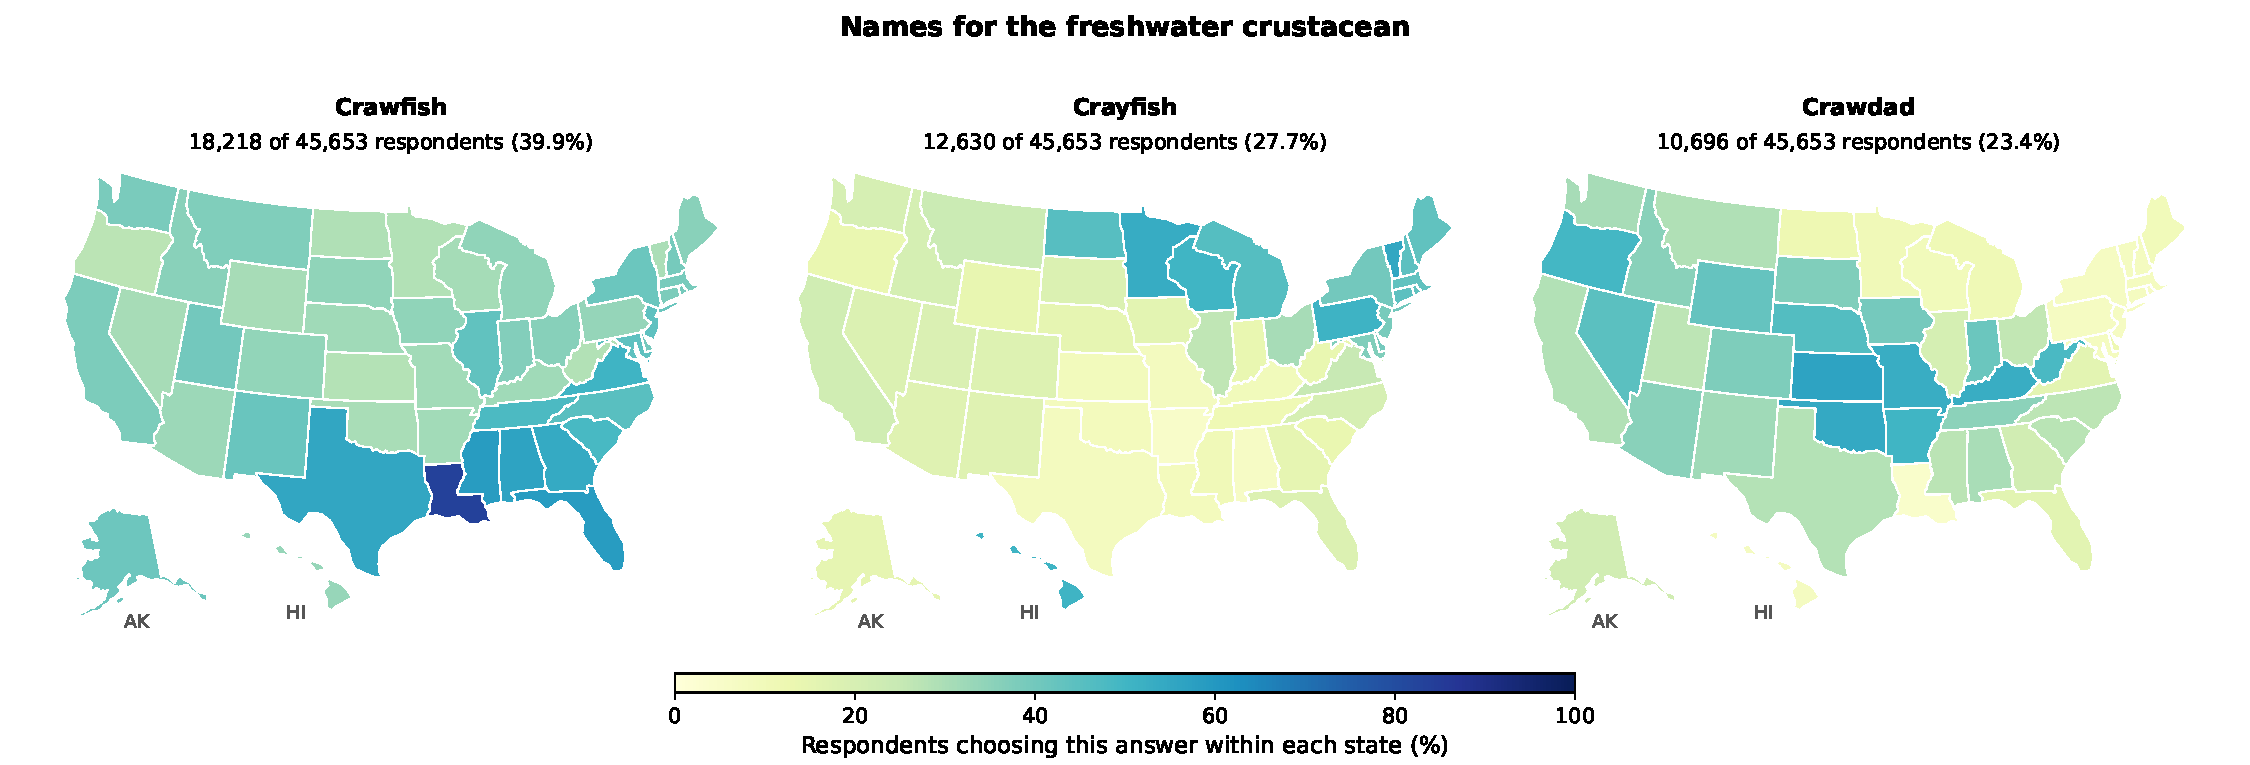
\includegraphics[width=\linewidth]{q66_response_maps.pdf}
\caption{Freshwater crustacean name distribution across states.}
\label{fig:q66}
\end{figure}

Crawfish is most common around the Gulf and Southeast, crayfish in the Northeast and Great Lakes, and crawdad in several central and inland states. The geograhy shows a clear regional pattern, with some overlap between the terms.

\begin{figure}[ht]
\centering
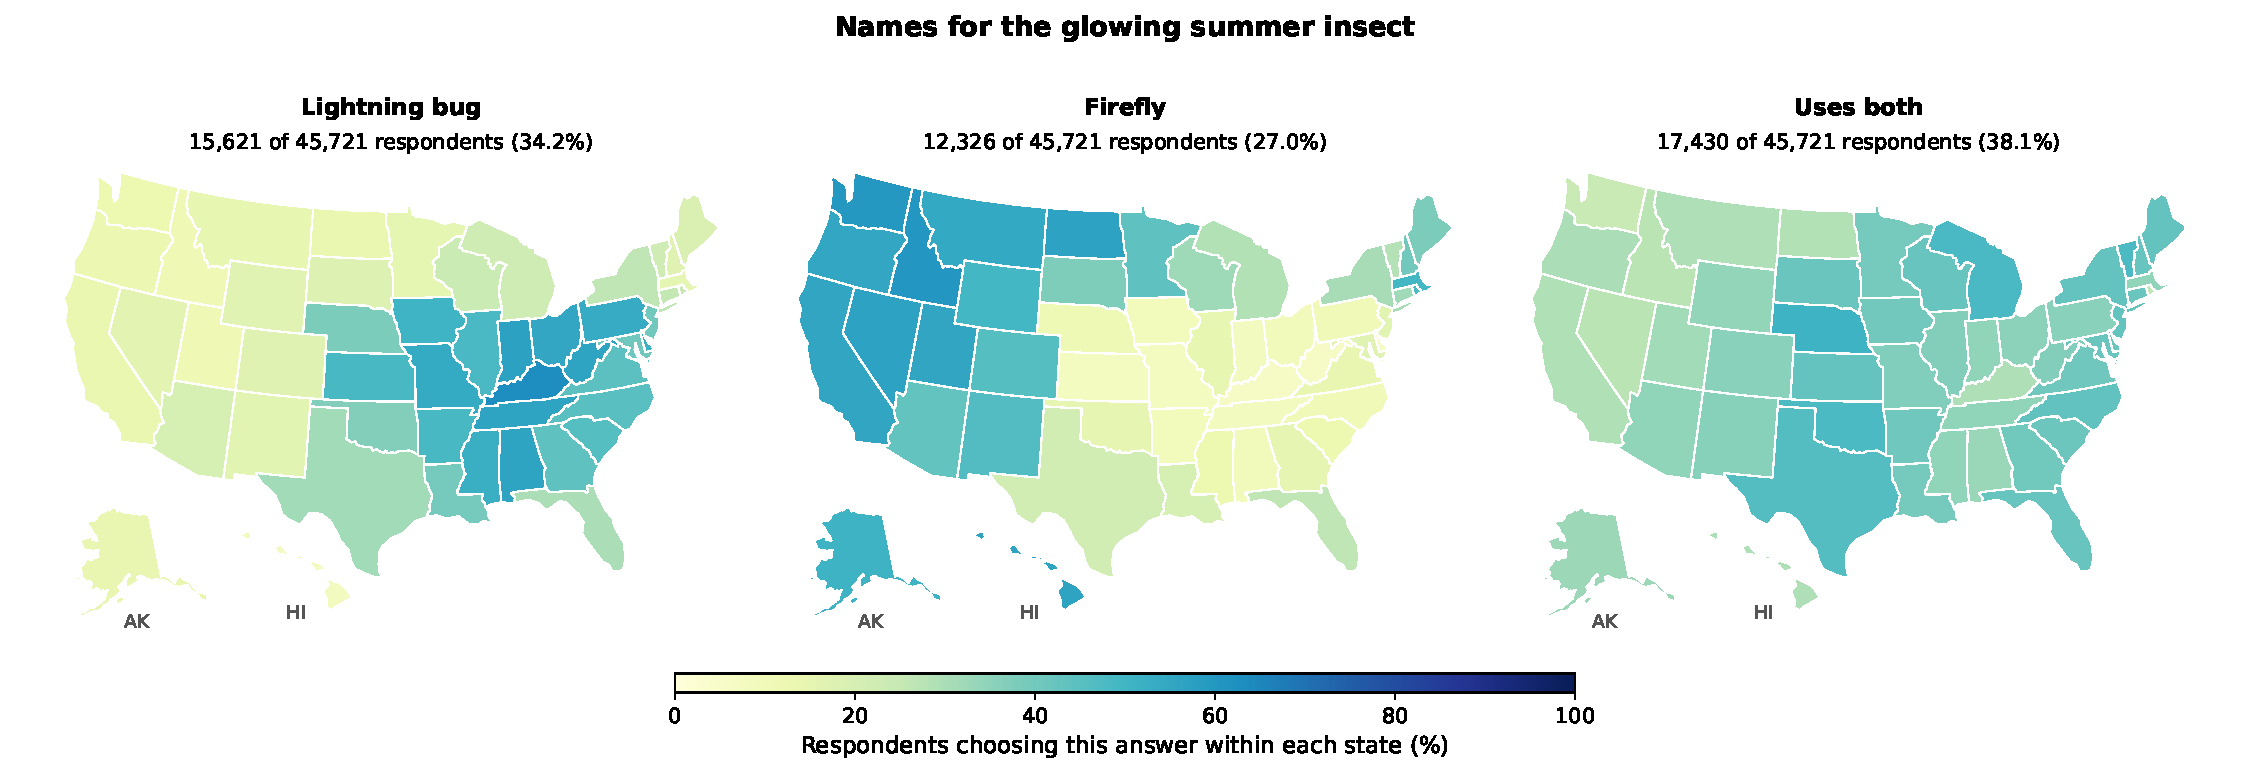
\includegraphics[width=\linewidth]{q65_response_maps.pdf}
\caption{Glowing summer insect distribution across states.}
\label{fig:q65}
\end{figure}

Lightning bug is more common in central and eastern states, while firefly is more common in the West. Also, many people across the entire country use both terms.

Q74 has more names that are common. Roly poly is common across much of the South and interior, potato bug stands out around Utah and parts of the Pacific Northwest, and doodle bug around Texas and Louisiana.

\begin{figure}[ht]
\centering
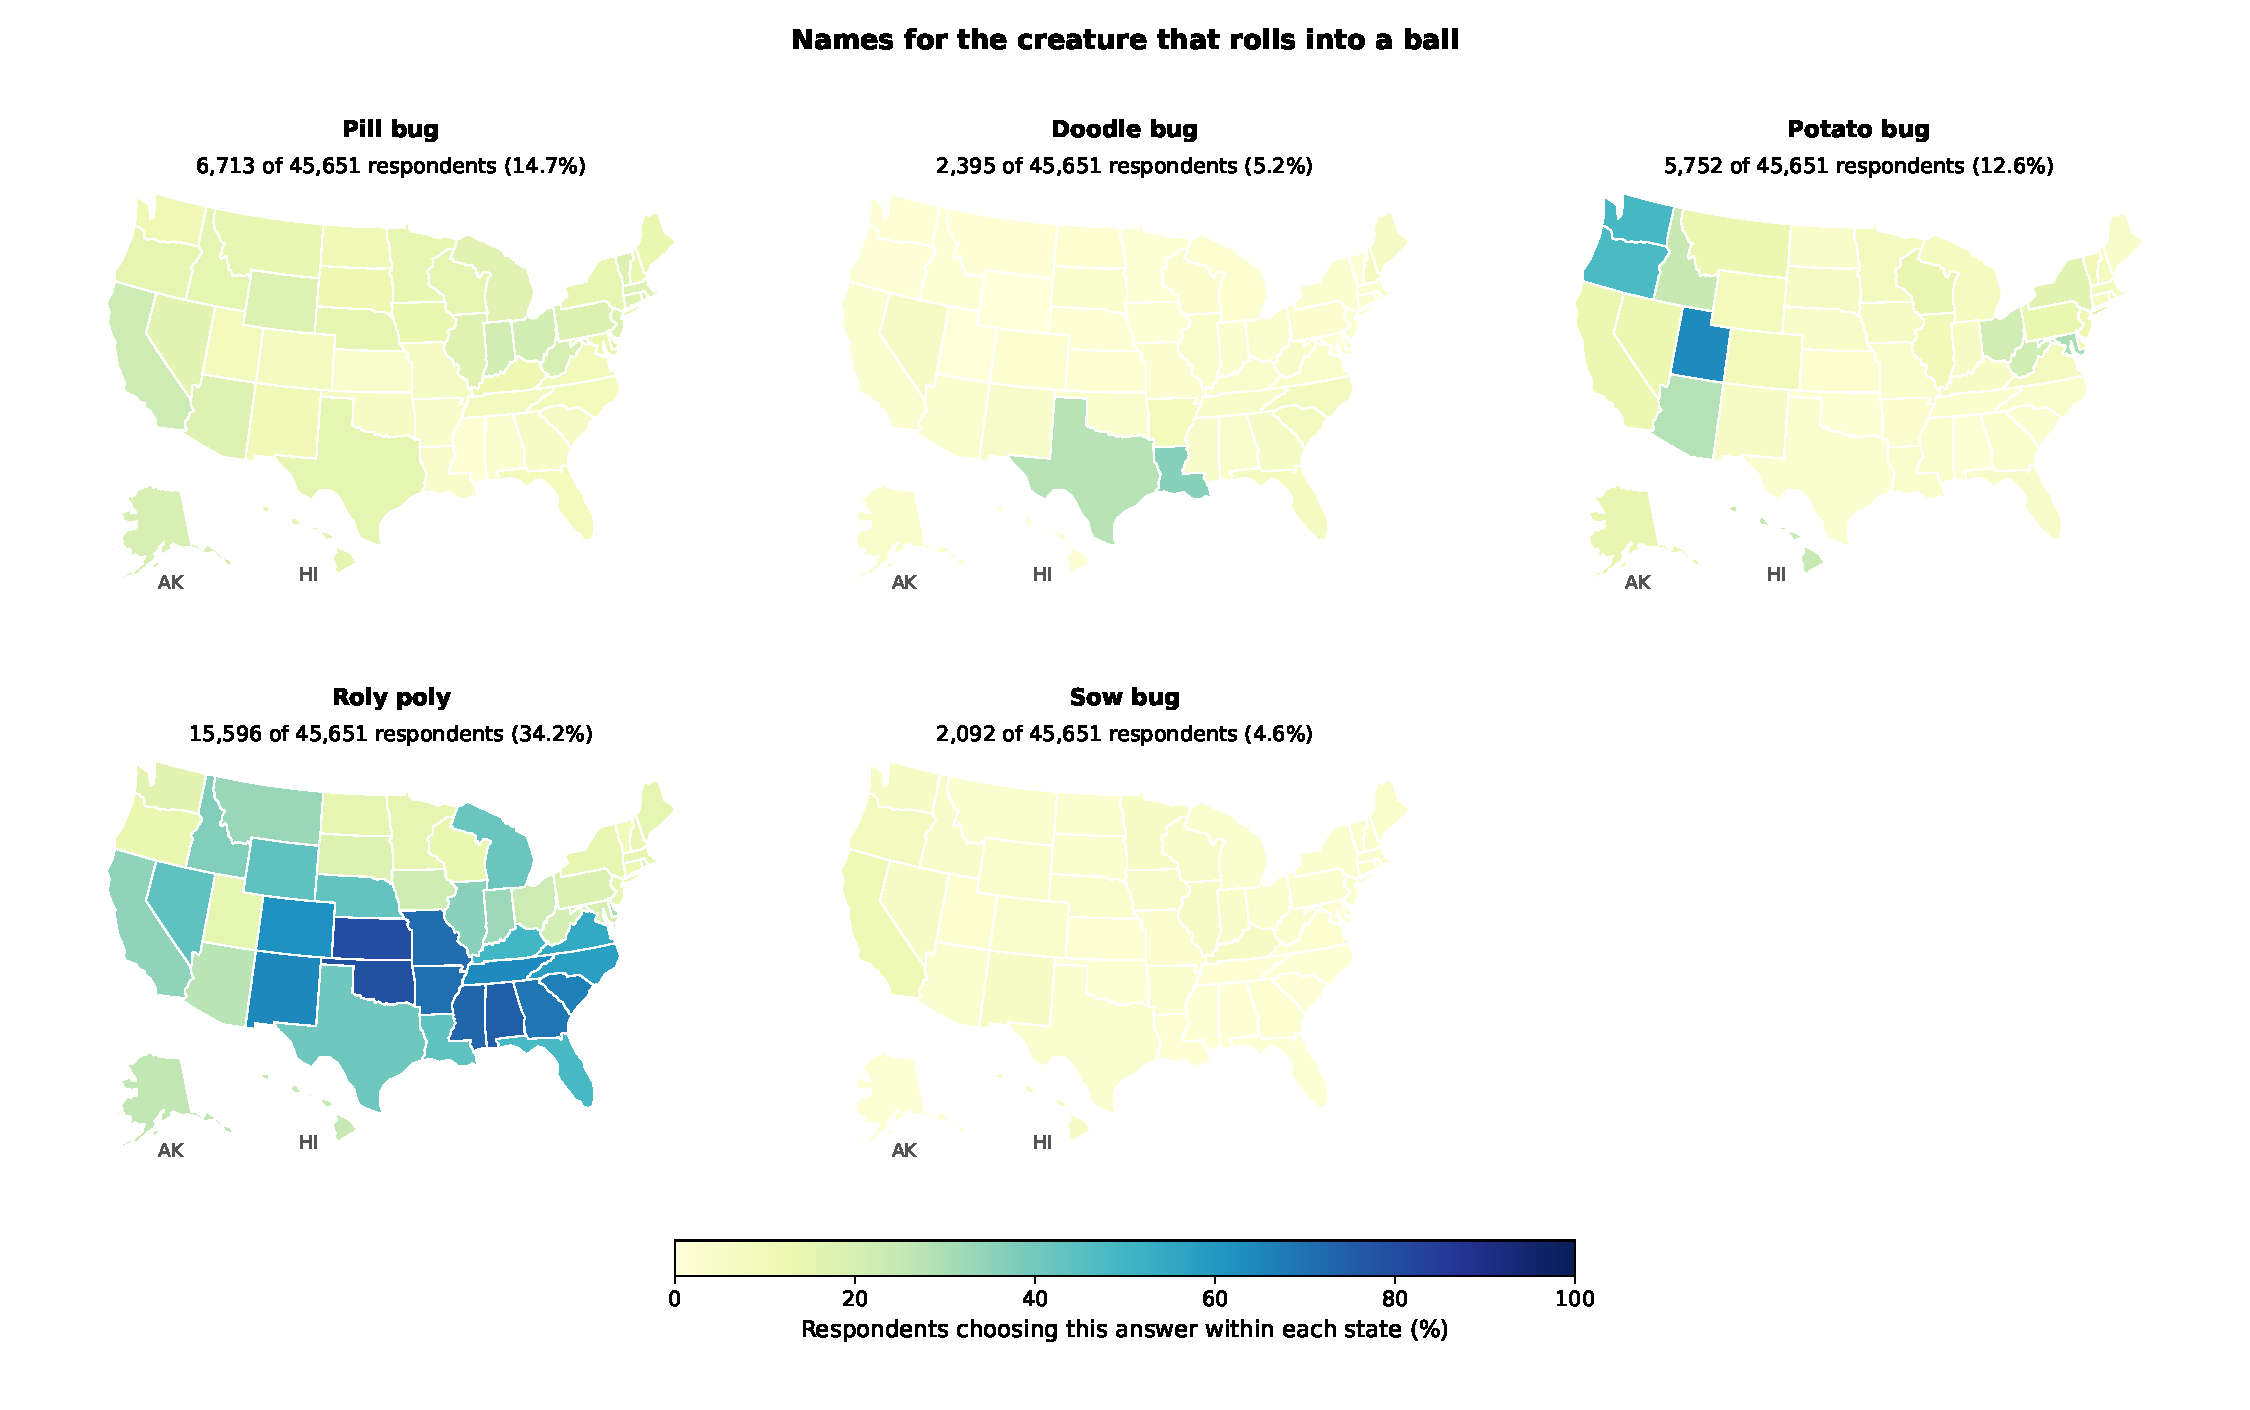
\includegraphics[width=\linewidth]{q74_response_maps.pdf}
\caption{Selected Q74 response shares.}
\label{fig:q74}
\end{figure}

Roly poly is used by 50.3\% of crawdad respondents and 20.6\% of crayfish respondents, a difference of 29.7 percentage points. Compared with 34.2\% overall, it is more common among crawdad respondents and less common among crayfish respondents. These percentages suggest that the answers to Q66 and Q74 are related.

\begin{figure}[ht]
\centering
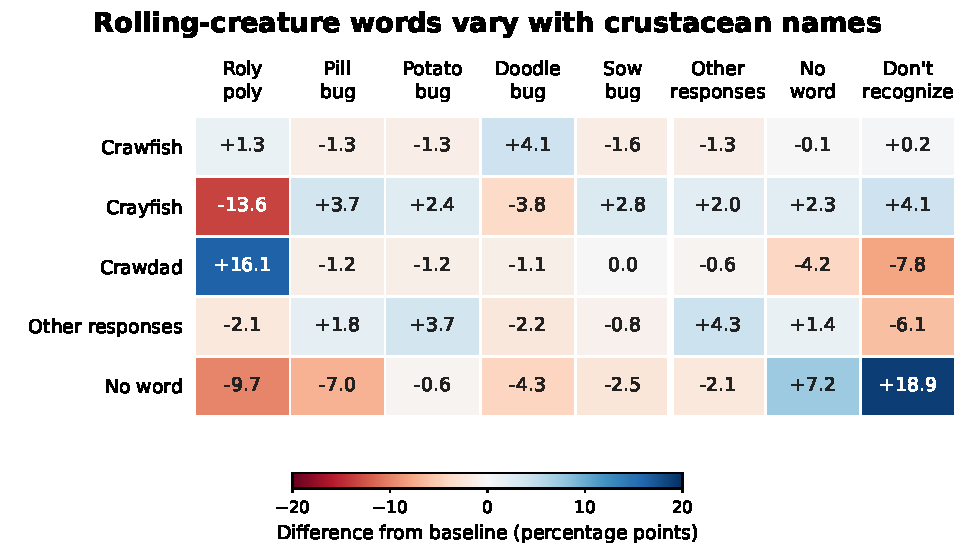
\includegraphics[width=\linewidth]{q66_q74_association.pdf}
\caption{Q74 percentages conditional on Q66, expressed as differences from the overall baseline.}
\label{fig:pair}
\end{figure}

\begin{figure}[ht]
\centering
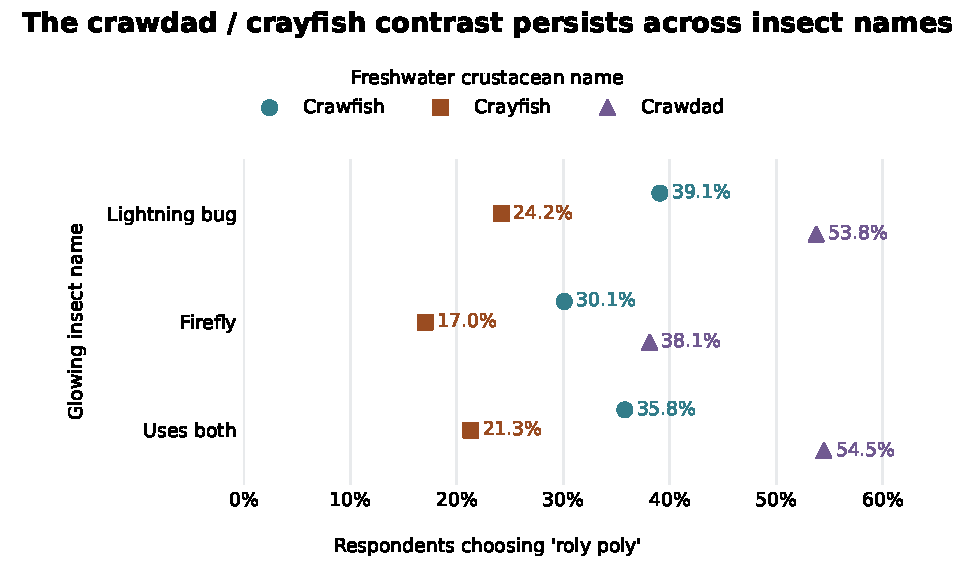
\includegraphics[width=\linewidth]{q65_q66_q74_association.pdf}
\caption{The roly poly percentage within selected Q65--Q66 groups.}
\label{fig:third}
\end{figure}

Crawdad respondents are more likely than crayfish respondents to use roly poly within each of the three shown Q65 groups. The percentages are 53.8\% and 24.2\% among lightning-bug respondents, and 38.1\% and 17.0\% among firefly respondents.

\section{Dimension Reduction}
Answer numbers are not measurements, so the difference between codes 1 and 4 have no size meaning. Therefore, a binary column for every answer choice is used. This gives 468 features for the 40,061 people who answered every question. Each person has one active feature per question.

PCA on centered data is compared with PCA on standardized data to see whether less common word choices reveal regional patterns that more common choices might hide.

\begin{center}
\begin{tabular}{lrrr}
\hline
Input & First PC & First two PCs & First 50 PCs\\
\hline
Centered binary & 4.04\% & 7.65\% & 56.30\%\\
Standardized binary & 1.93\% & 3.59\% & 29.86\%\\
\hline
\end{tabular}
\end{center}

\begin{figure}[ht]
\centering
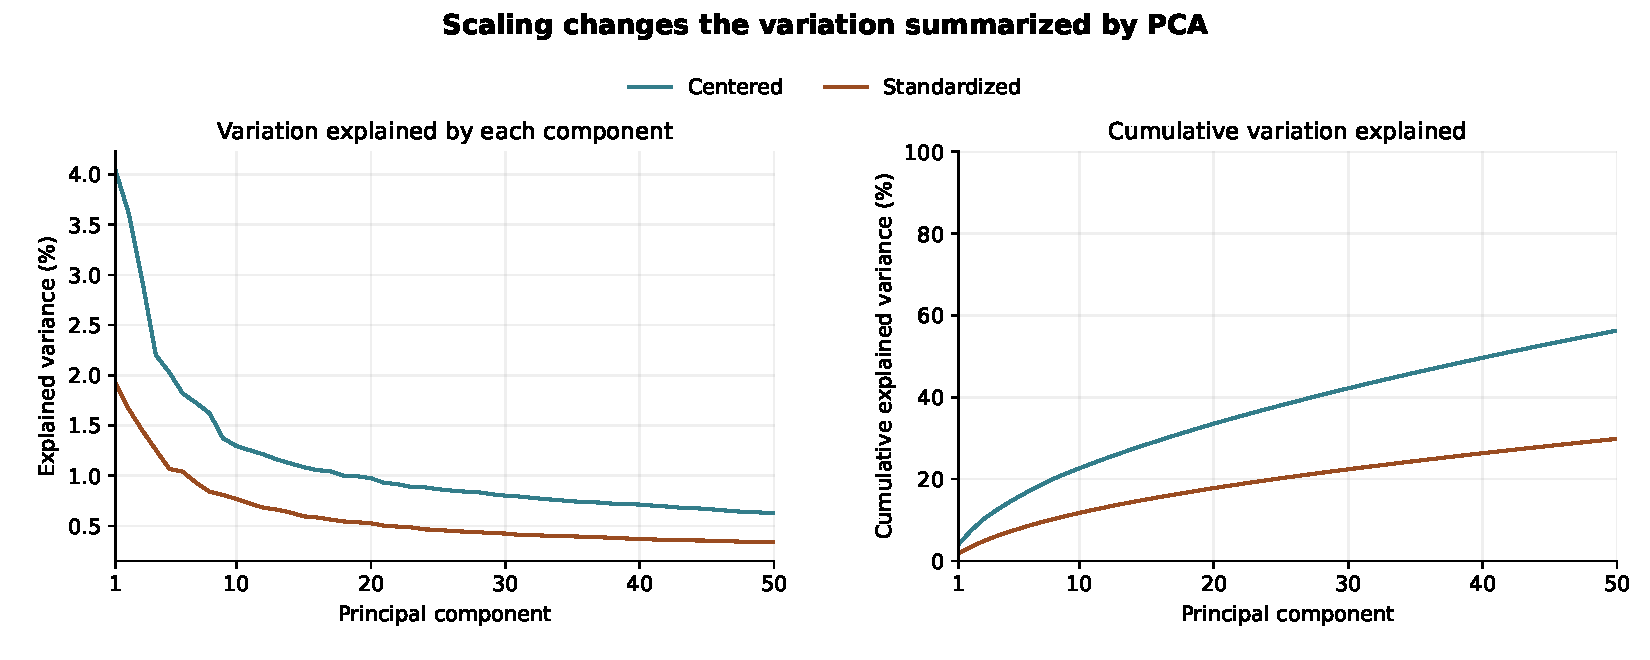
\includegraphics[width=\linewidth]{step3_pca_variance.pdf}
\caption{Explained variation under the two feature treatments.}
\label{fig:variance}
\end{figure}

50 components from centered PCA are used for the later analysis. These retain 56.30\% of the variation in respondents' answers. This reduces the size of the data, but some differences between respondents are lost.

\begin{figure}[ht]
\centering
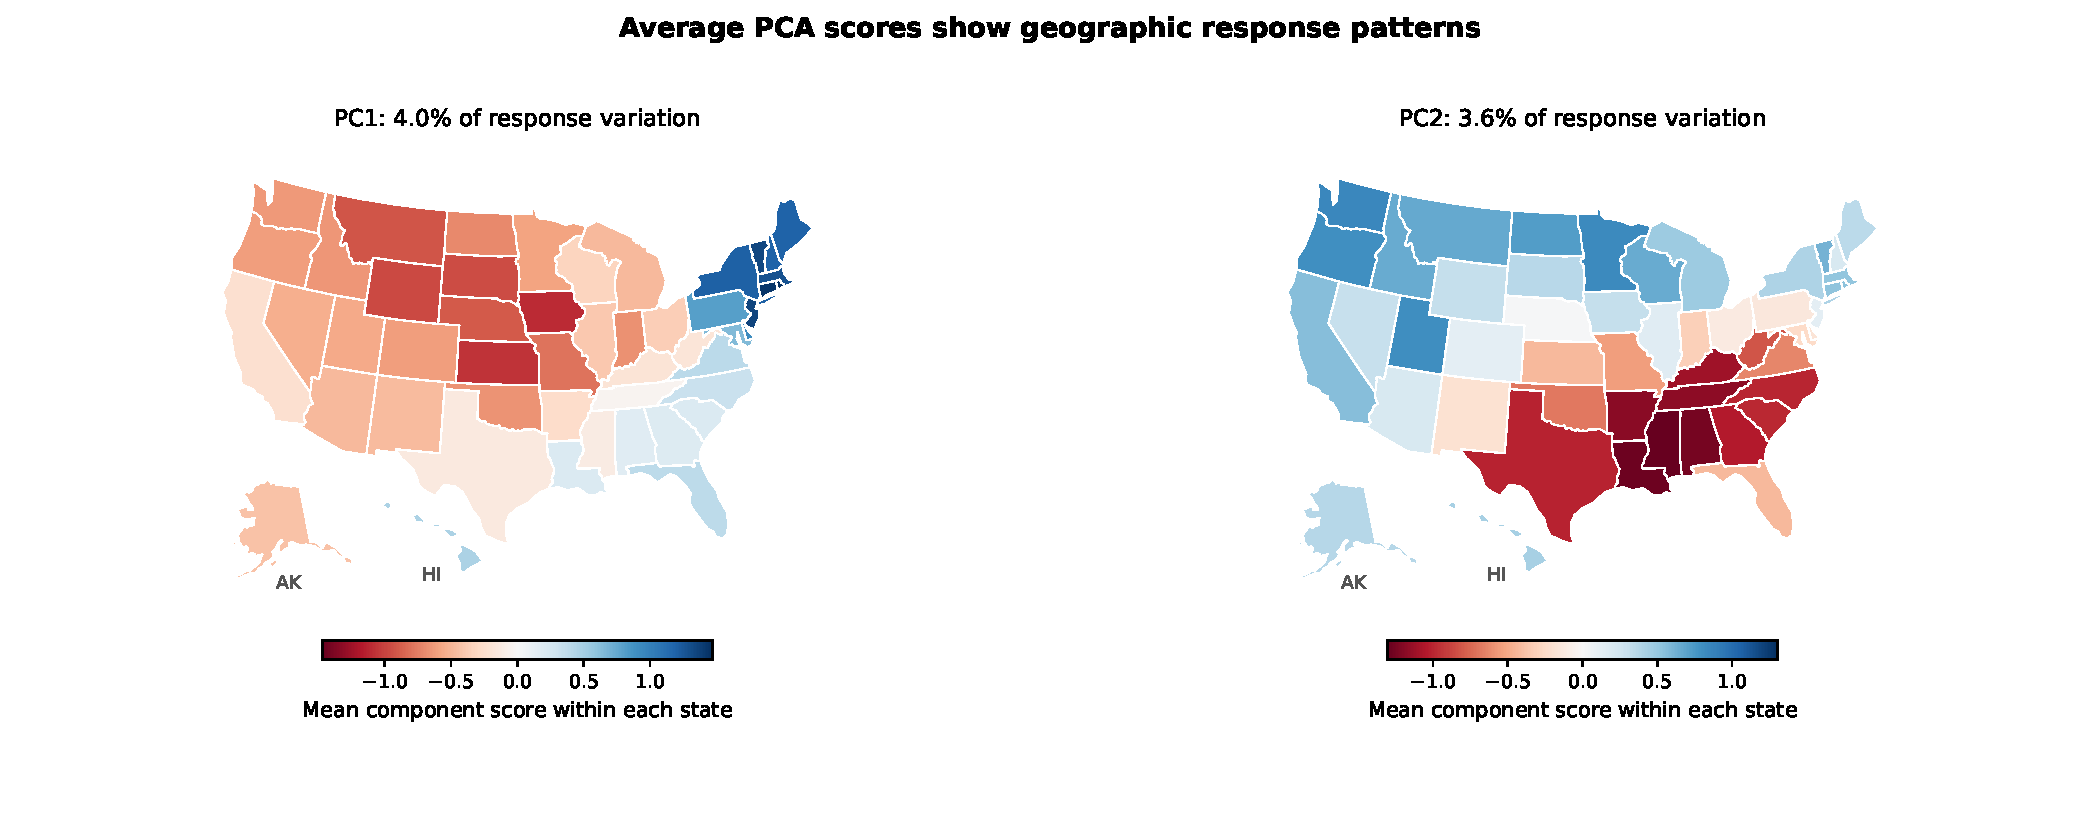
\includegraphics[width=\linewidth]{step3_pca_score_maps.pdf}
\caption{Mean centered PC1 and PC2 scores within states.}
\label{fig:pca-maps}
\end{figure}

PC1 contrasts sneakers and soda with tennis shoes and pop. Its state averages are higher in much of the Northeast. PC2 contrasts kitty-corner and firefly with catty-corner, y'all, and coke, and is generally lower in the South.

The geographic plots suggest that word choices vary by region, but the regions do not form clearly seperate groups. PC1--PC2 and PC2--PC3 show different parts of this variation, so the interpretation depends on which components are plotted. Scaling changes the patterns too. These plots suggest gradual regional differences rather than hard regional separation.

\begin{figure}[ht]
\centering
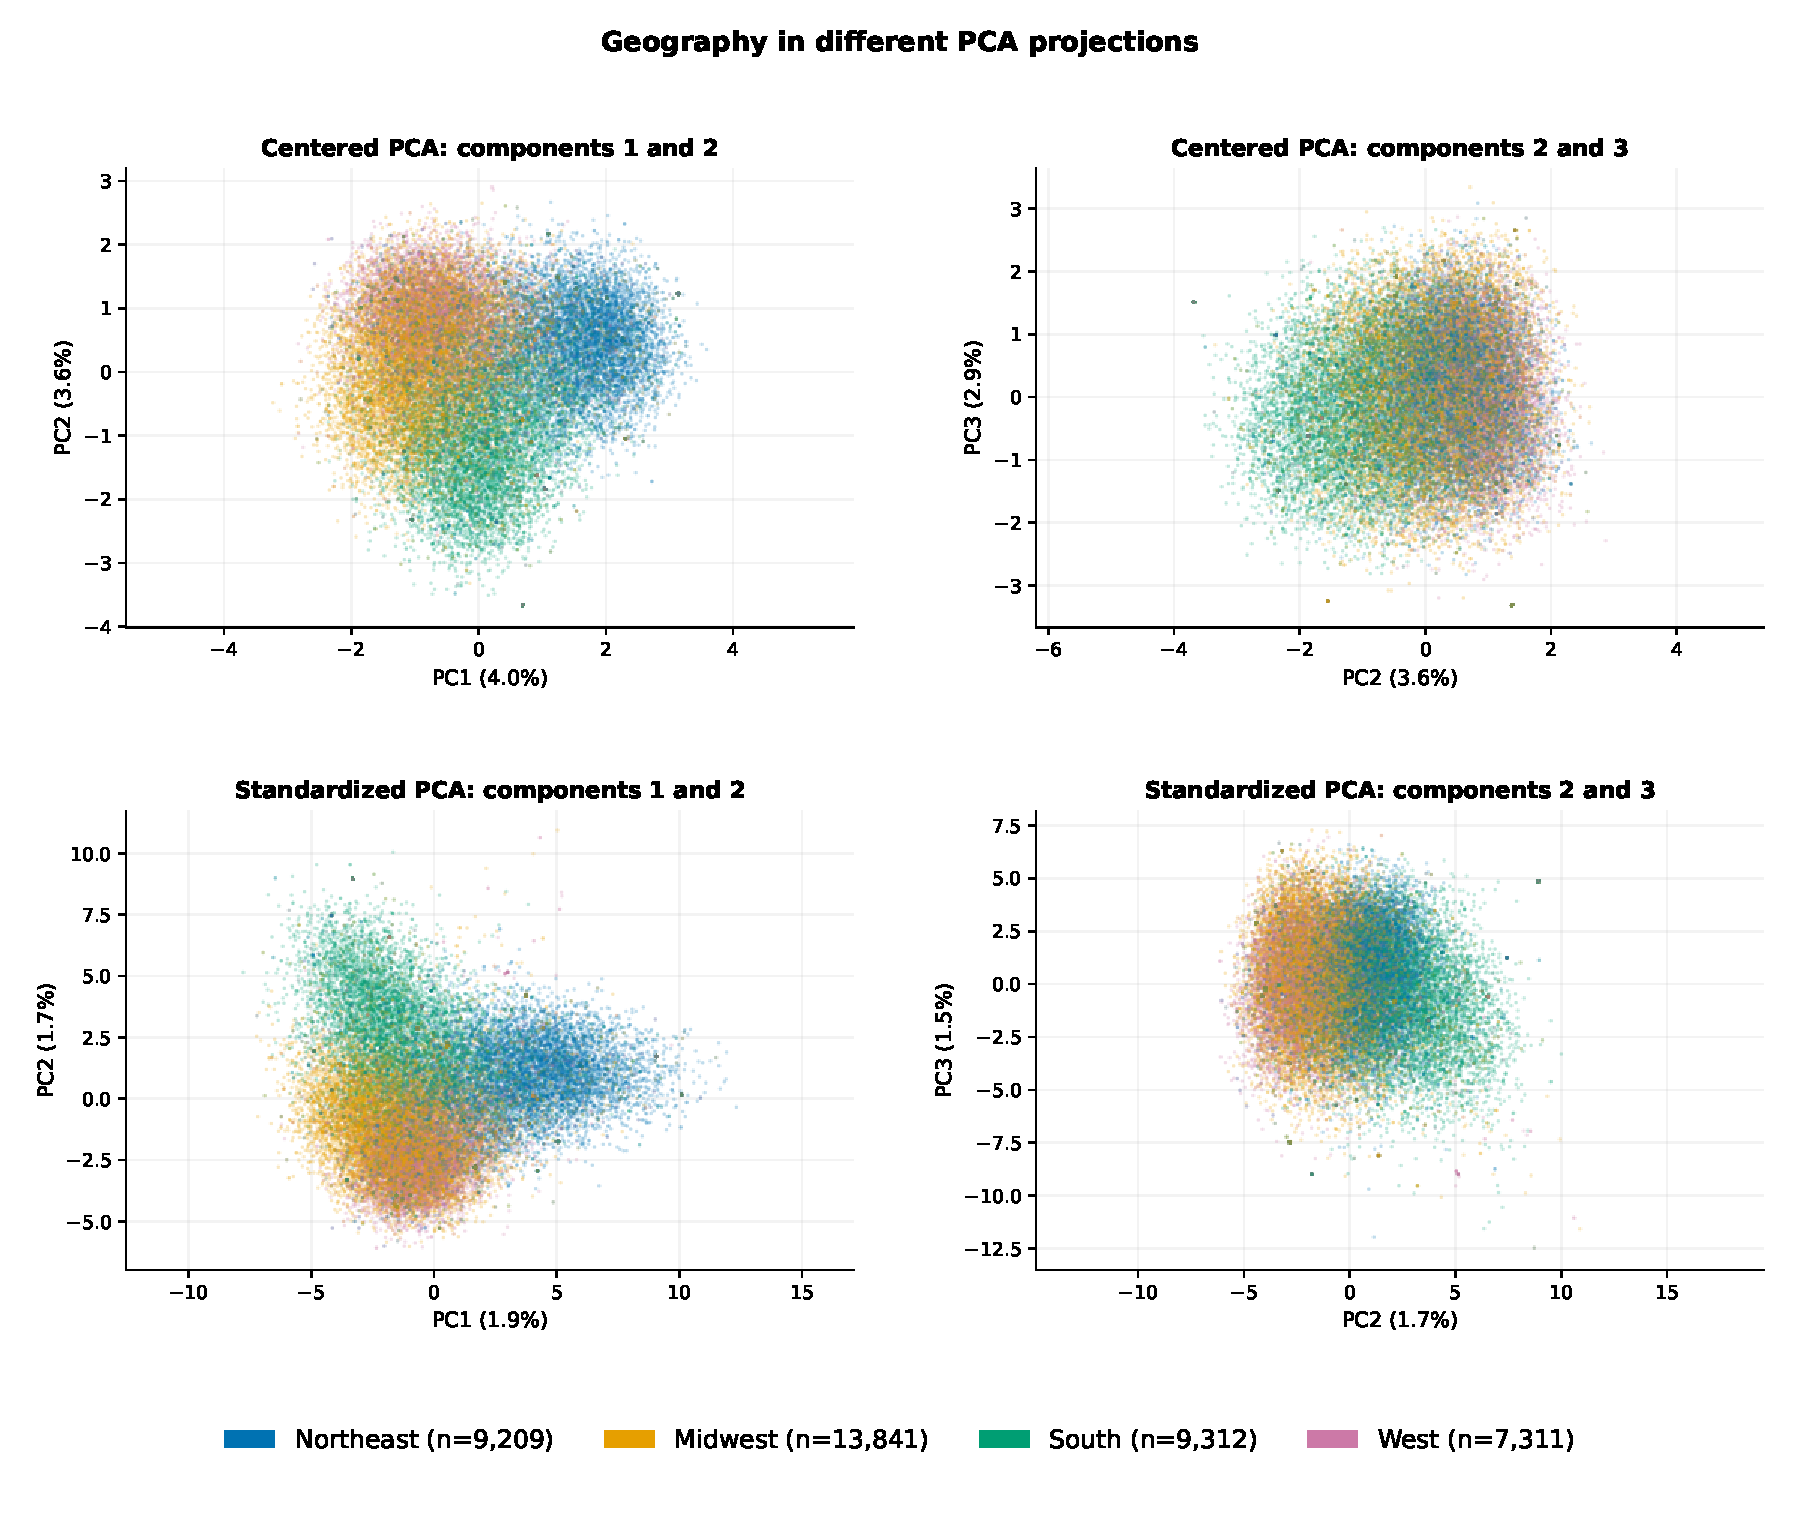
\includegraphics[width=\linewidth]{step3_pca_geography.pdf}
\caption{Centered and standardized PCA in two coordinate pairs, colored by location.}
\label{fig:pca-geography}
\end{figure}

I also use t-SNE on the centered PCA scores, with perplexities 30 and 50, the same seed, PCA initialization, and 1,000 iterations. Both plots are very similar and show geographic patterns, with a lot of Midwest--West mixing.

\begin{figure}[ht]
\centering
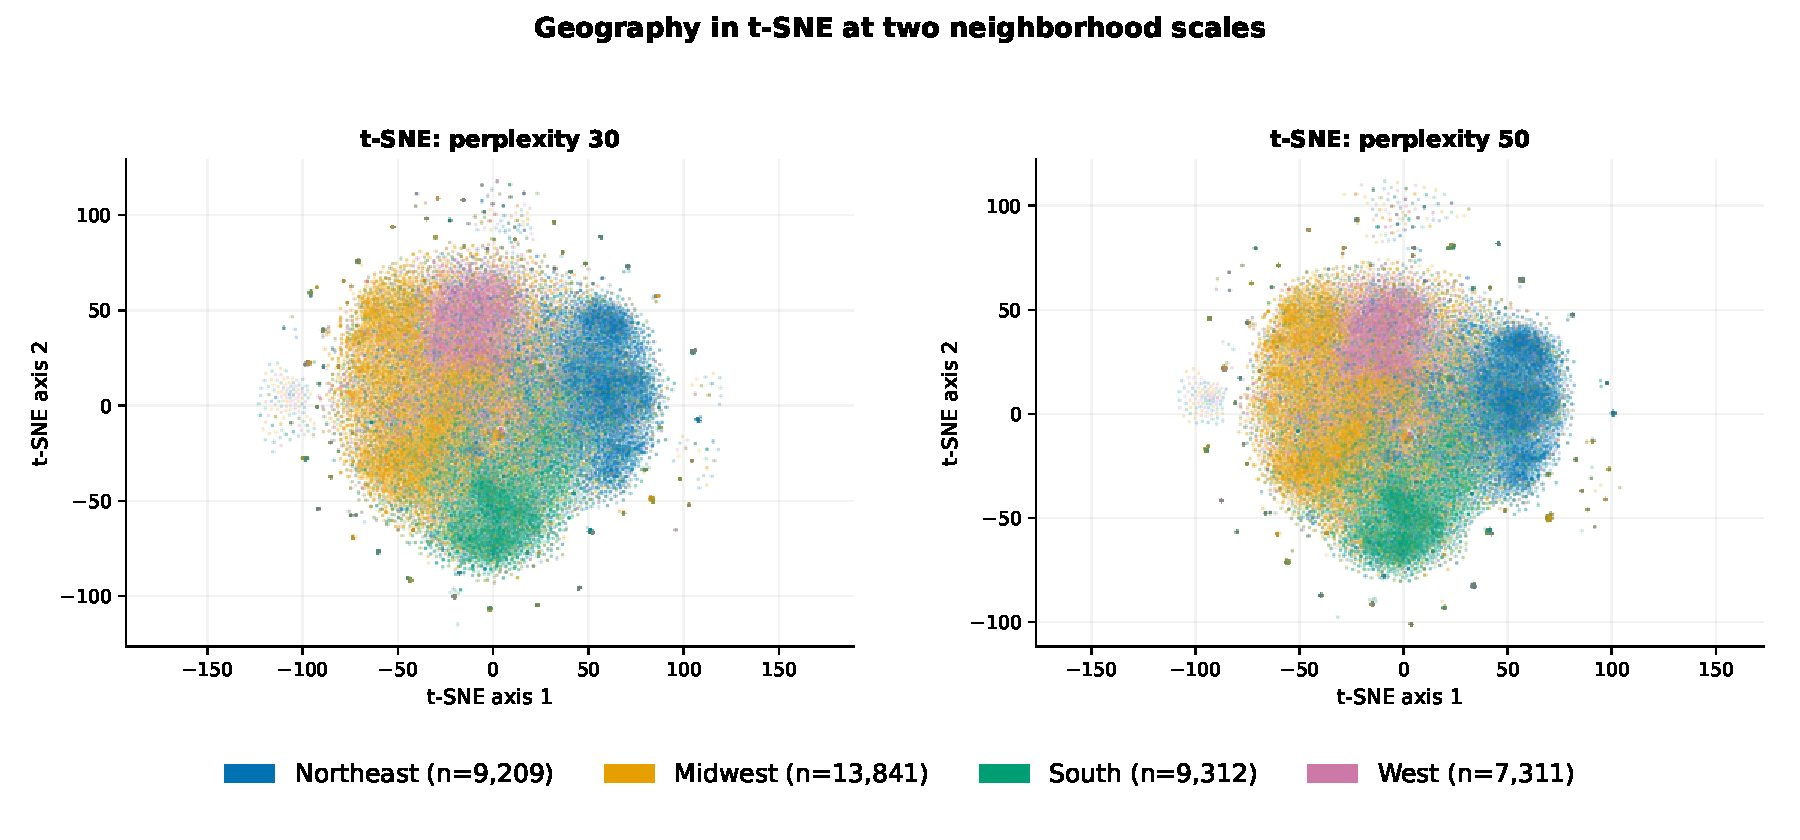
\includegraphics[width=\linewidth]{step3_tsne_geography.pdf}
\caption{t-SNE at two perplexities.}
\label{fig:tsne}
\end{figure}

\section{Clustering}
For clustering analysis, K-means and a Gaussian mixture model were fitted to the same centered PCA scores mentioned before. This lets me compare the formed clusters with their actual geography.

\begin{figure}[ht]
\centering
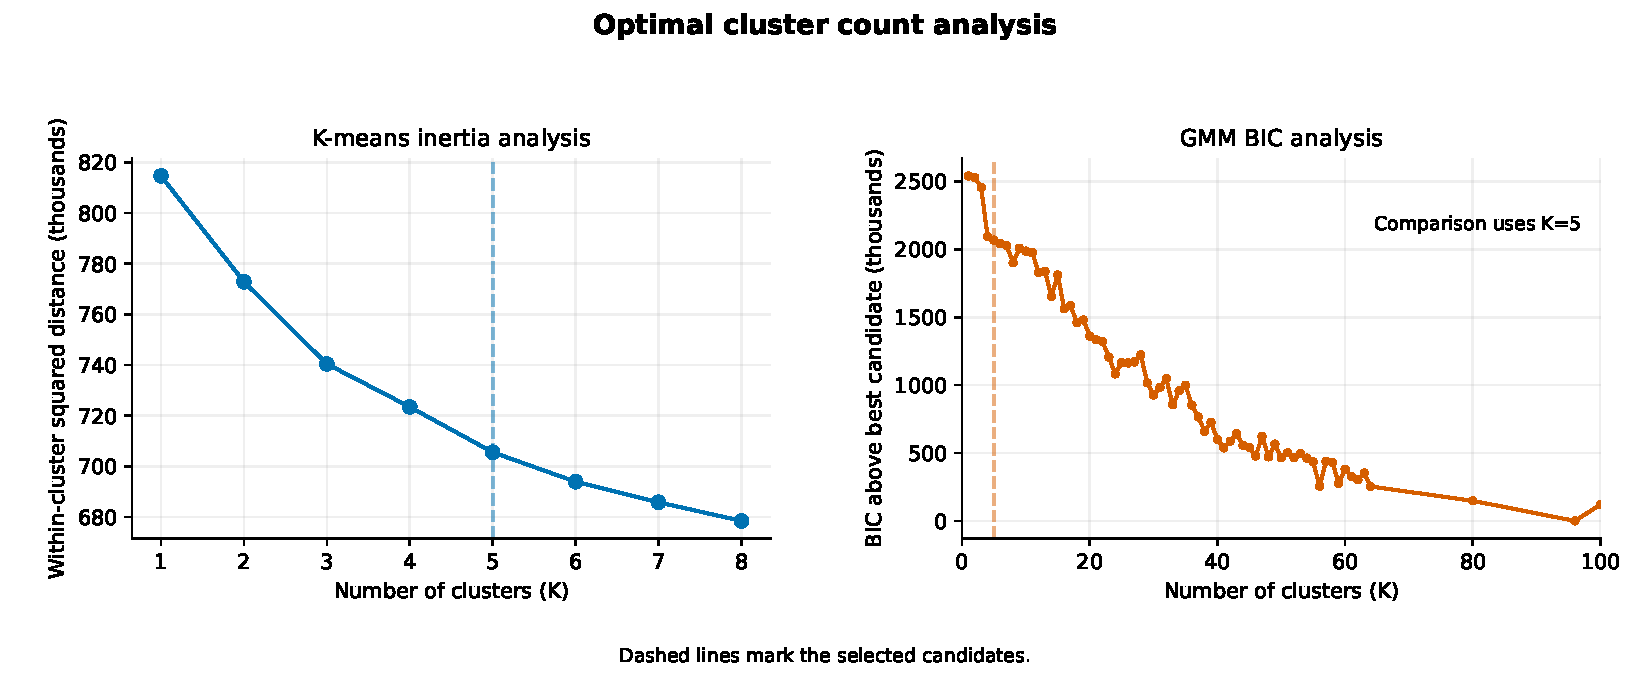
\includegraphics[width=\linewidth]{step4_cluster_selection.pdf}
\caption{K-means inertia and GMM BIC across tested counts.}
\label{fig:k}
\end{figure}

I try 1--8 K-means groups and 1--64, 80, 96, and 100 GMM components. K-means inertia falls without a clear elbow at five. The lowest tested GMM BIC is at 96 components, about 1,096,173, compared with 3,164,478 at five. This is only the best of the tested counts.

I use five groups to have an equivalent comparison. The group sizes already show that the methods divide the same people differently.

\begin{center}
\begin{tabular}{lrrrrr}
\hline
Method & C1 & C2 & C3 & C4 & C5\\
\hline
K-means & 8,778 & 11,053 & 9,790 & 637 & 9,803\\
GMM & 4,863 & 24,373 & 1,100 & 635 & 9,090\\
\hline
\end{tabular}
\end{center}

\subsection{Comparing the partitions}
The plots show overlapping clouds. K-means has four large clusters and one small cluster, with C3 and C2 overlapping, while GMM has three large clusters and two small clusters, hiding the large group overlap that was apparent in K-means. These plots only show a small part of the variation used for fitting.

\begin{figure}[ht]
\centering
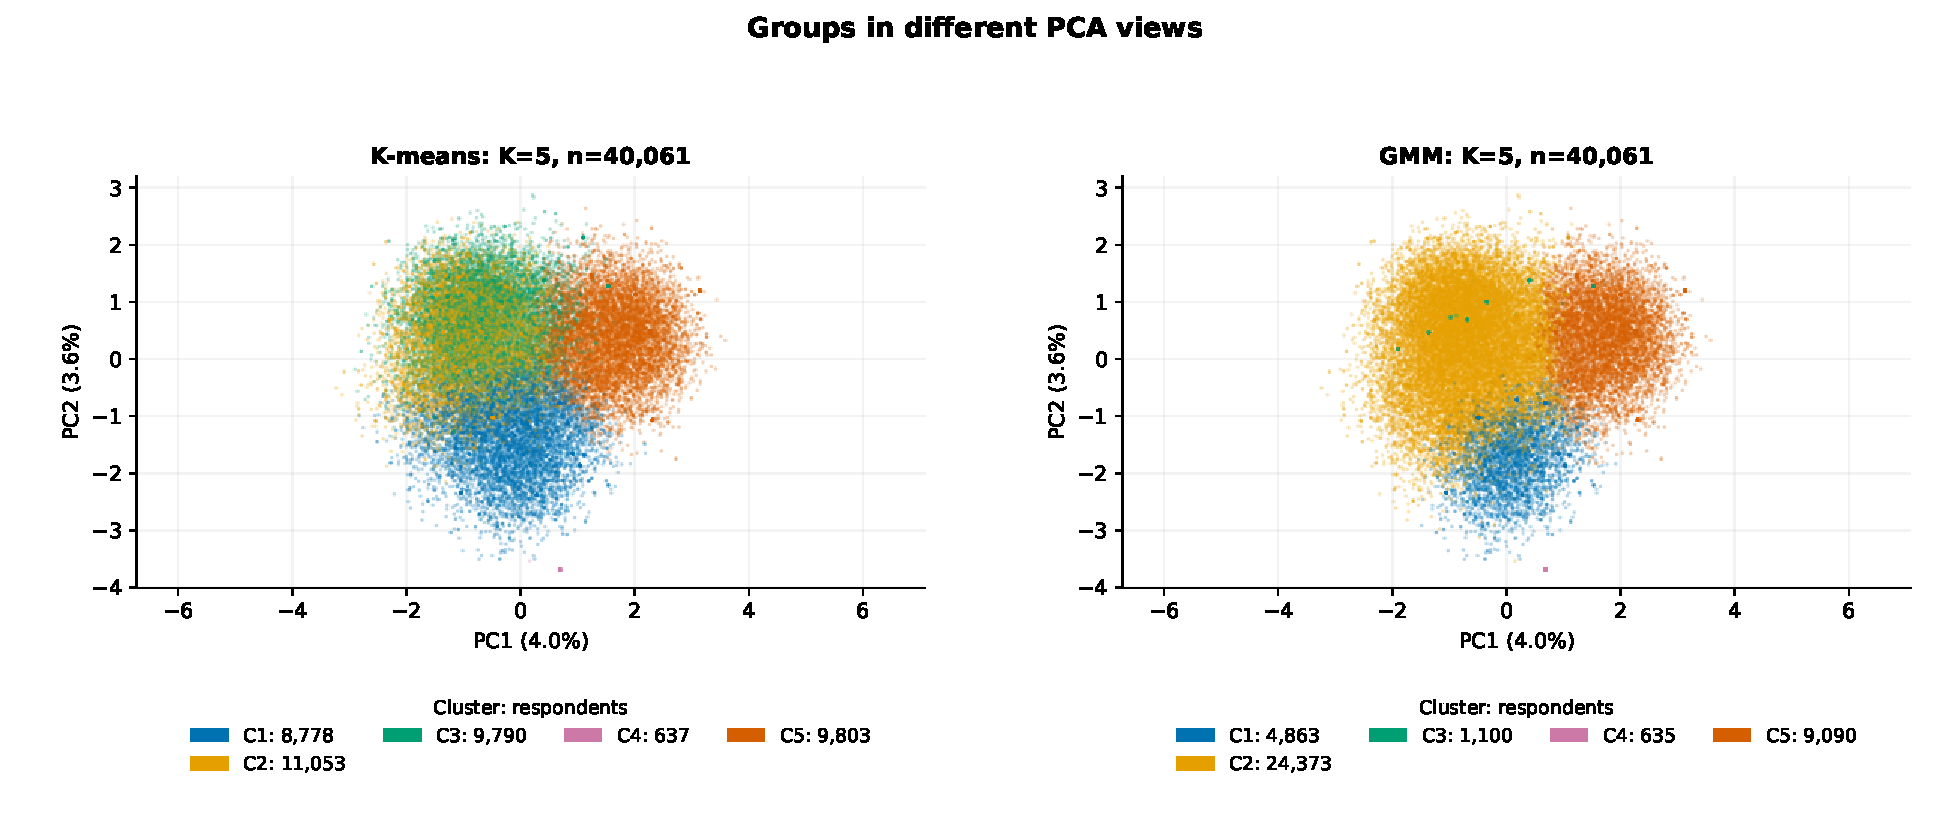
\includegraphics[width=\linewidth]{step4_clusters_pc1_pc2.pdf}
\caption{K-means and GMM clusters in PC1--PC2 coordinates.}
\label{fig:clusters12}
\end{figure}

\begin{figure}[ht]
\centering
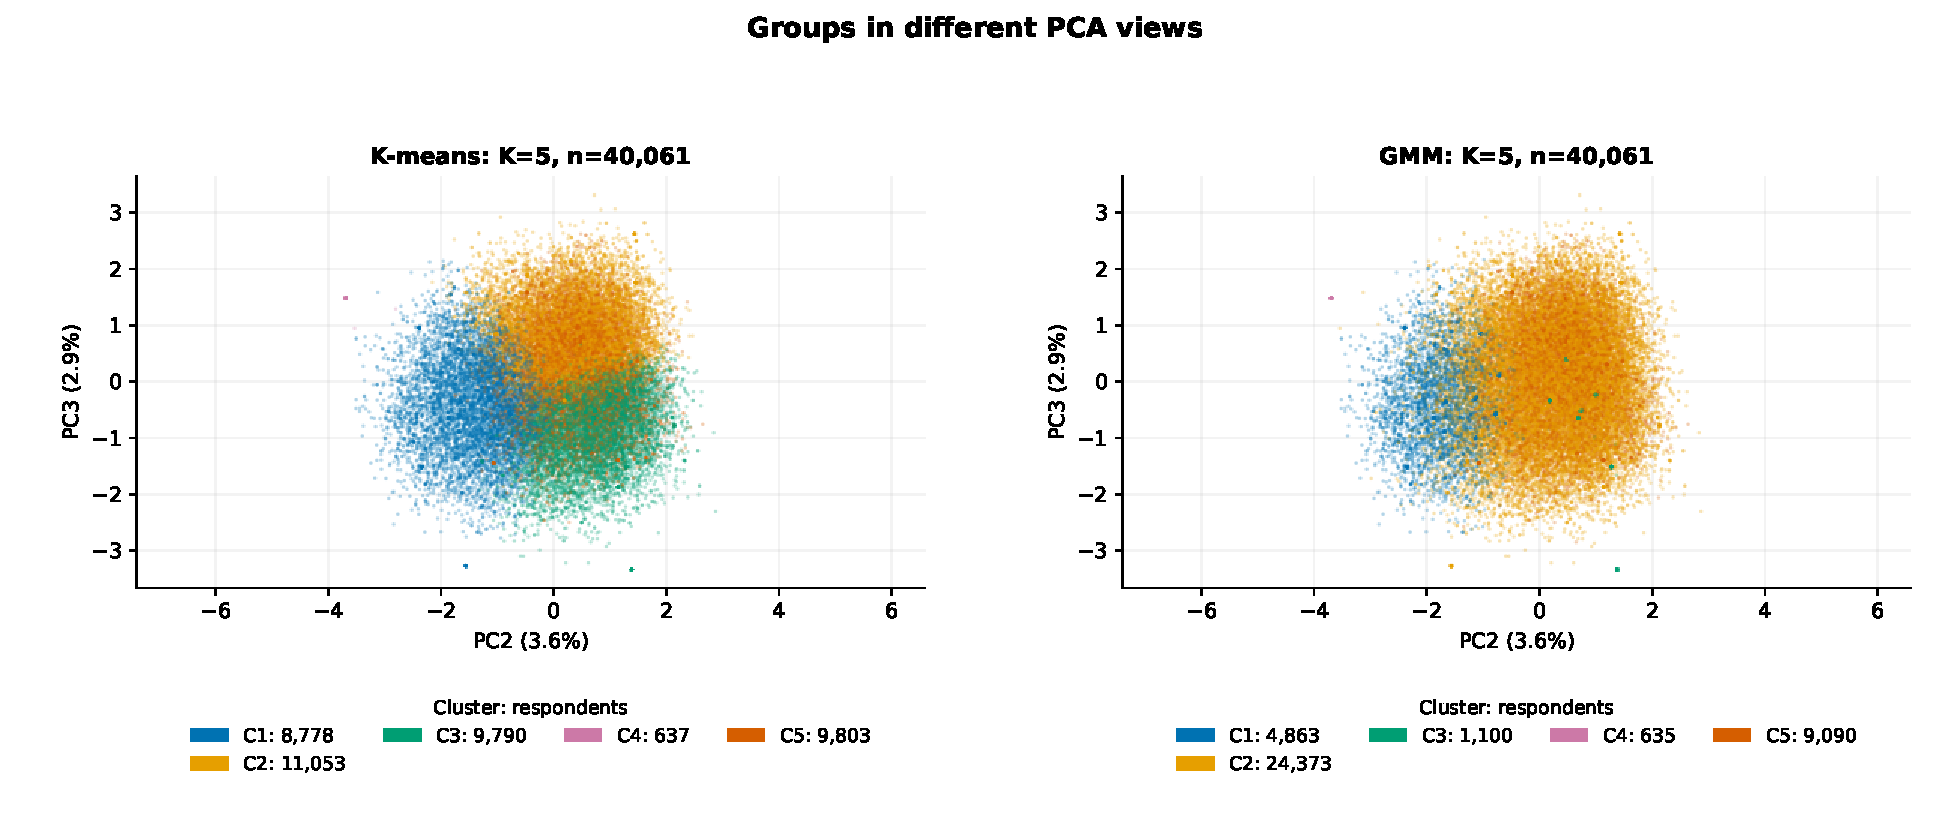
\includegraphics[width=\linewidth]{step4_clusters_pc2_pc3.pdf}
\caption{K-means and GMM clusters in PC2--PC3 coordinates.}
\label{fig:clusters23}
\end{figure}

\begin{figure}[ht]
\centering
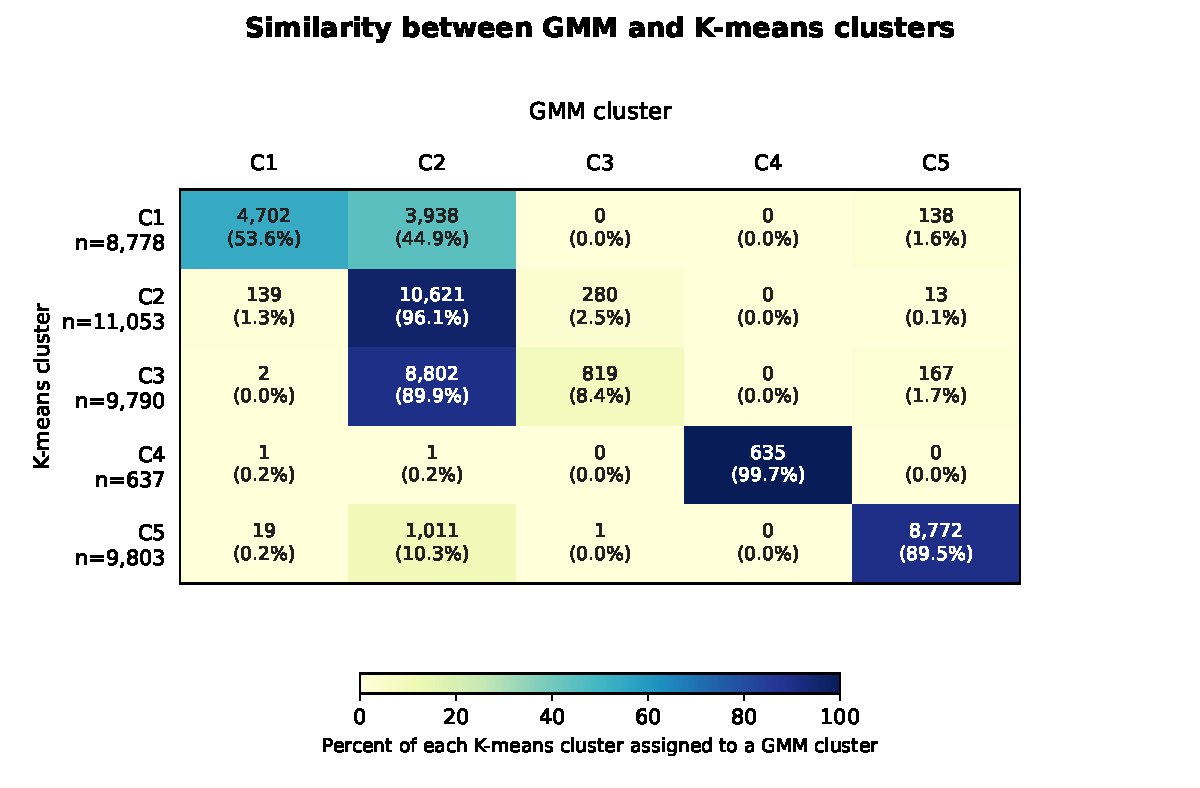
\includegraphics[width=\linewidth]{step4_cluster_agreement.pdf}
\caption{Comparison of cluster assignments.}
\label{fig:agreement}
\end{figure}

K-means and GMM agree on some groups, but produce different divisions overall. GMM C2 contains 96.1\% of K-means C2 and 89.9\% of K-means C3, largely combining these two groups. Meanwhile, 89.5\% of K-means C5 goes to GMM C5. The adjusted Rand index of 0.362 also shows that the two methods only partly agree.

\subsection{Geographic interpretation}
Both methods find a group common in the Northeast and another common in the South. K-means puts 69.3\% of eligible Northeast respondents in C5 and 54.4\% of South respondents in C1. GMM puts 66.7\% of Northeast respondents in C4 and 36.3\% of South respondents in C3. K-means divides Midwest and West respondents between C2 and C3, while GMM puts 84.2\% of Midwest and 84.7\% of West respondents in C2. Both methods broadly find similar geographic divisions. The main difference is that K-means splits much of the Midwest and West between two groups, while GMM largely combines these respondents in one.

\begin{figure}[ht]
\centering
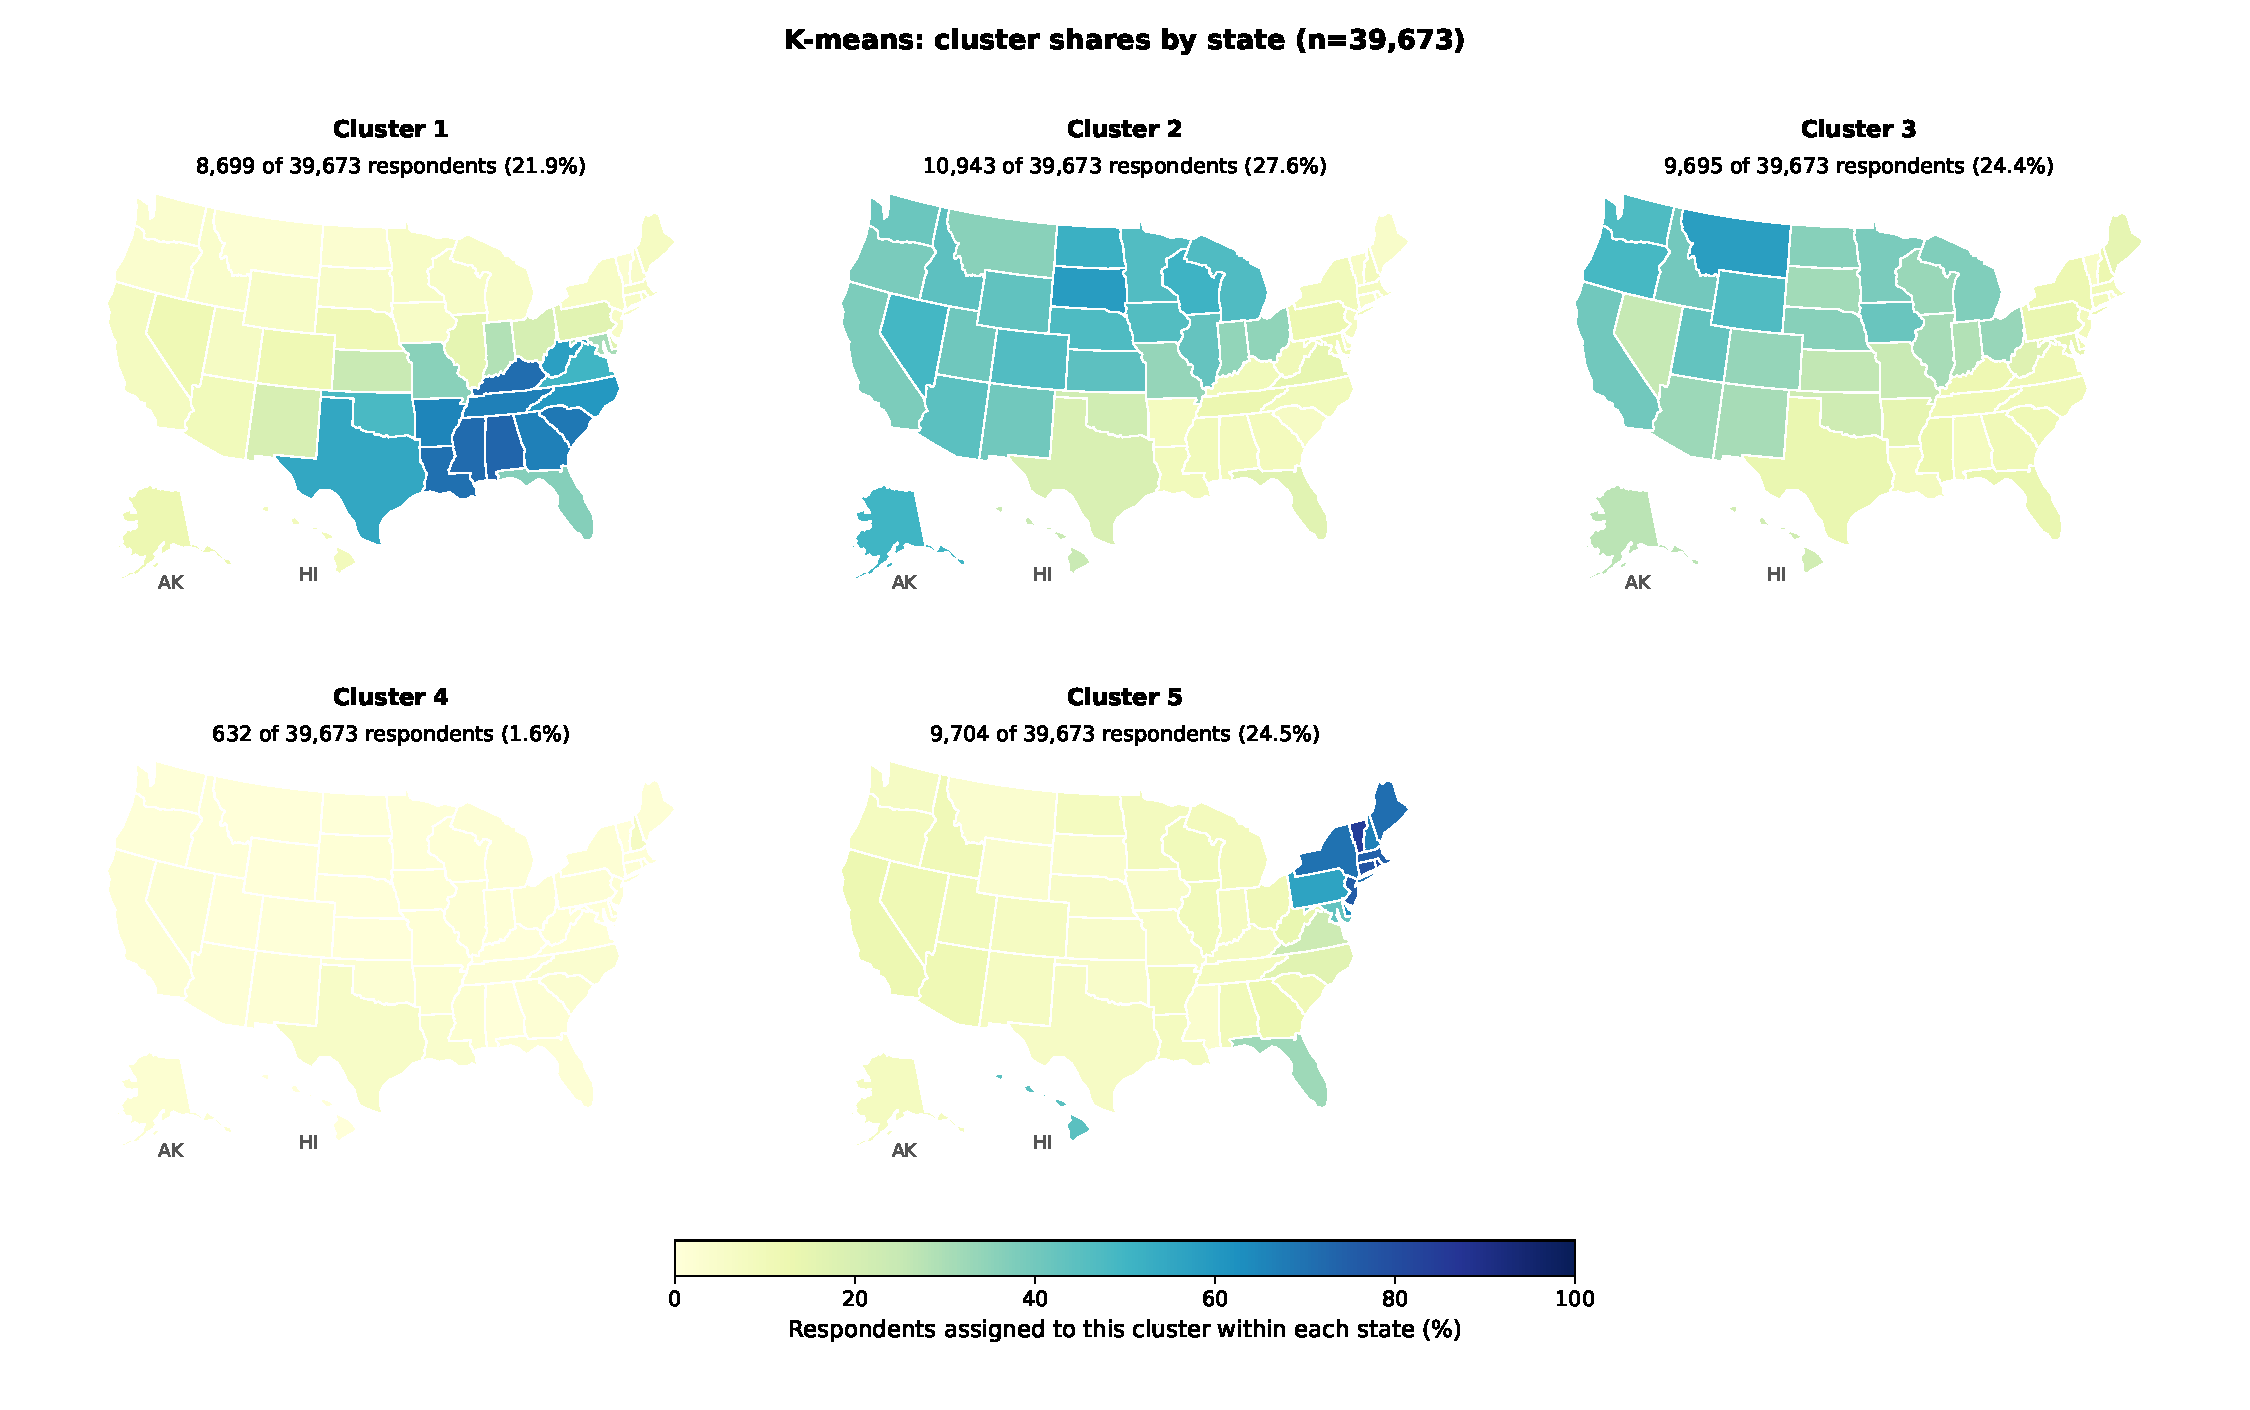
\includegraphics[width=\linewidth]{step4_kmeans_state_maps.pdf}
\caption{K-means clusters across states.}
\label{fig:kmeans-map}
\end{figure}

\begin{figure}[ht]
\centering
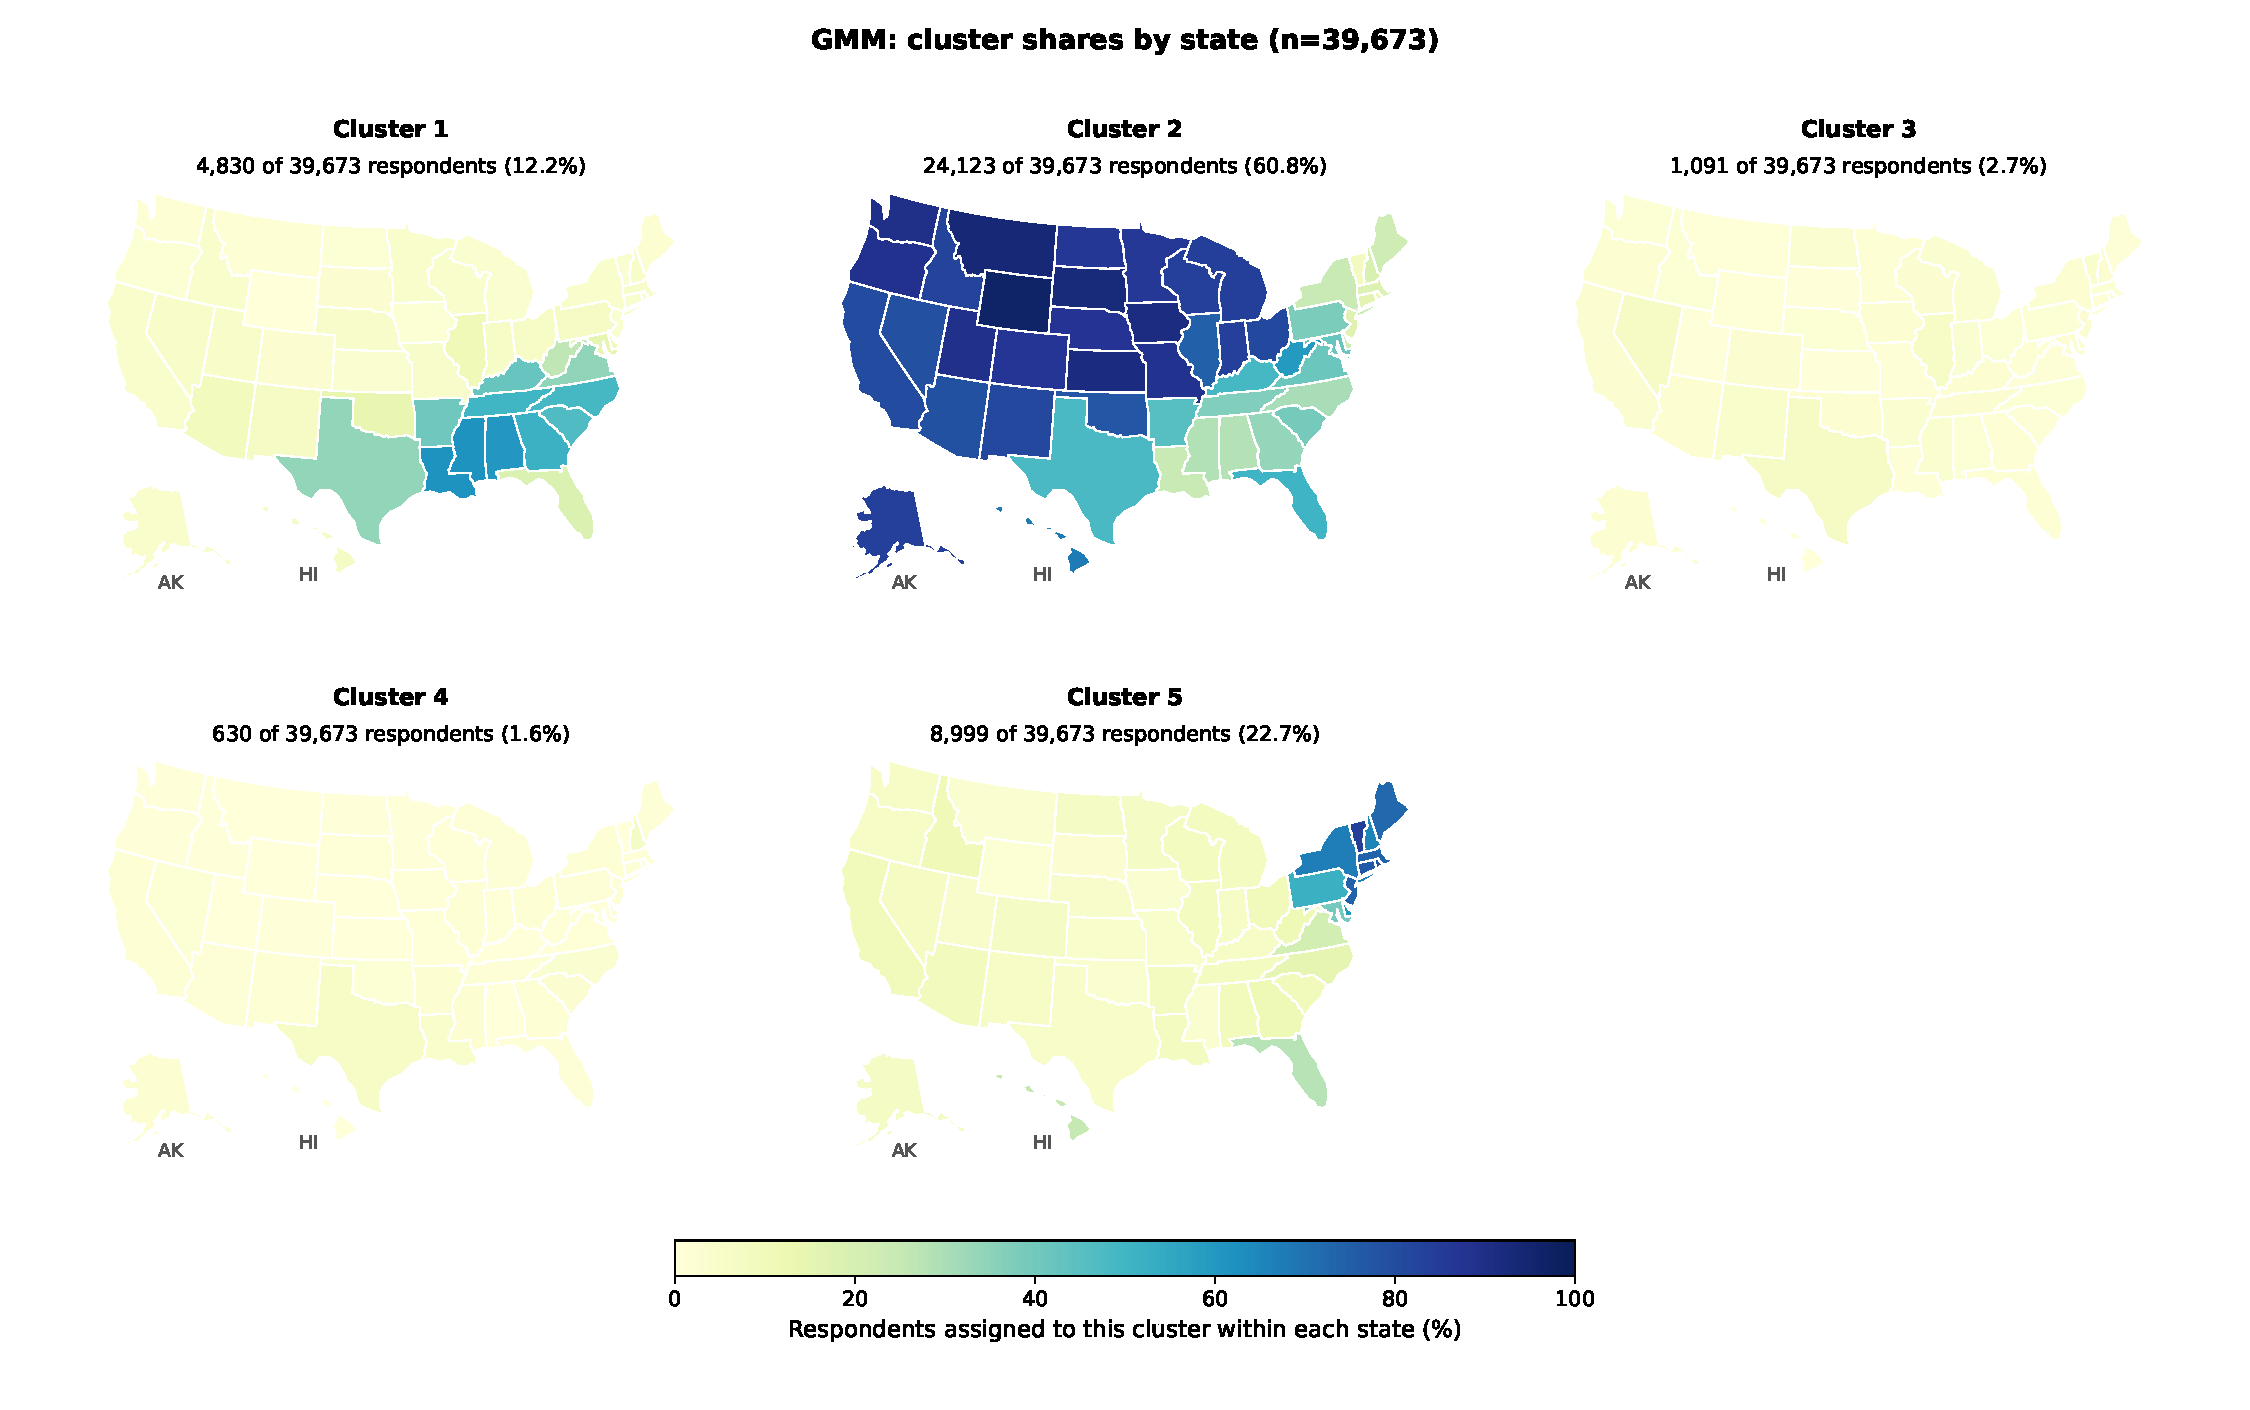
\includegraphics[width=\linewidth]{step4_gmm_state_maps.pdf}
\caption{GMM clusters across states.}
\label{fig:gmm-map}
\end{figure}

\subsection{Answers distinguishing K-means groups}
Each clusters answer percentages are compared with the percentages for all complete respondents.

\begin{figure}[ht]
\centering
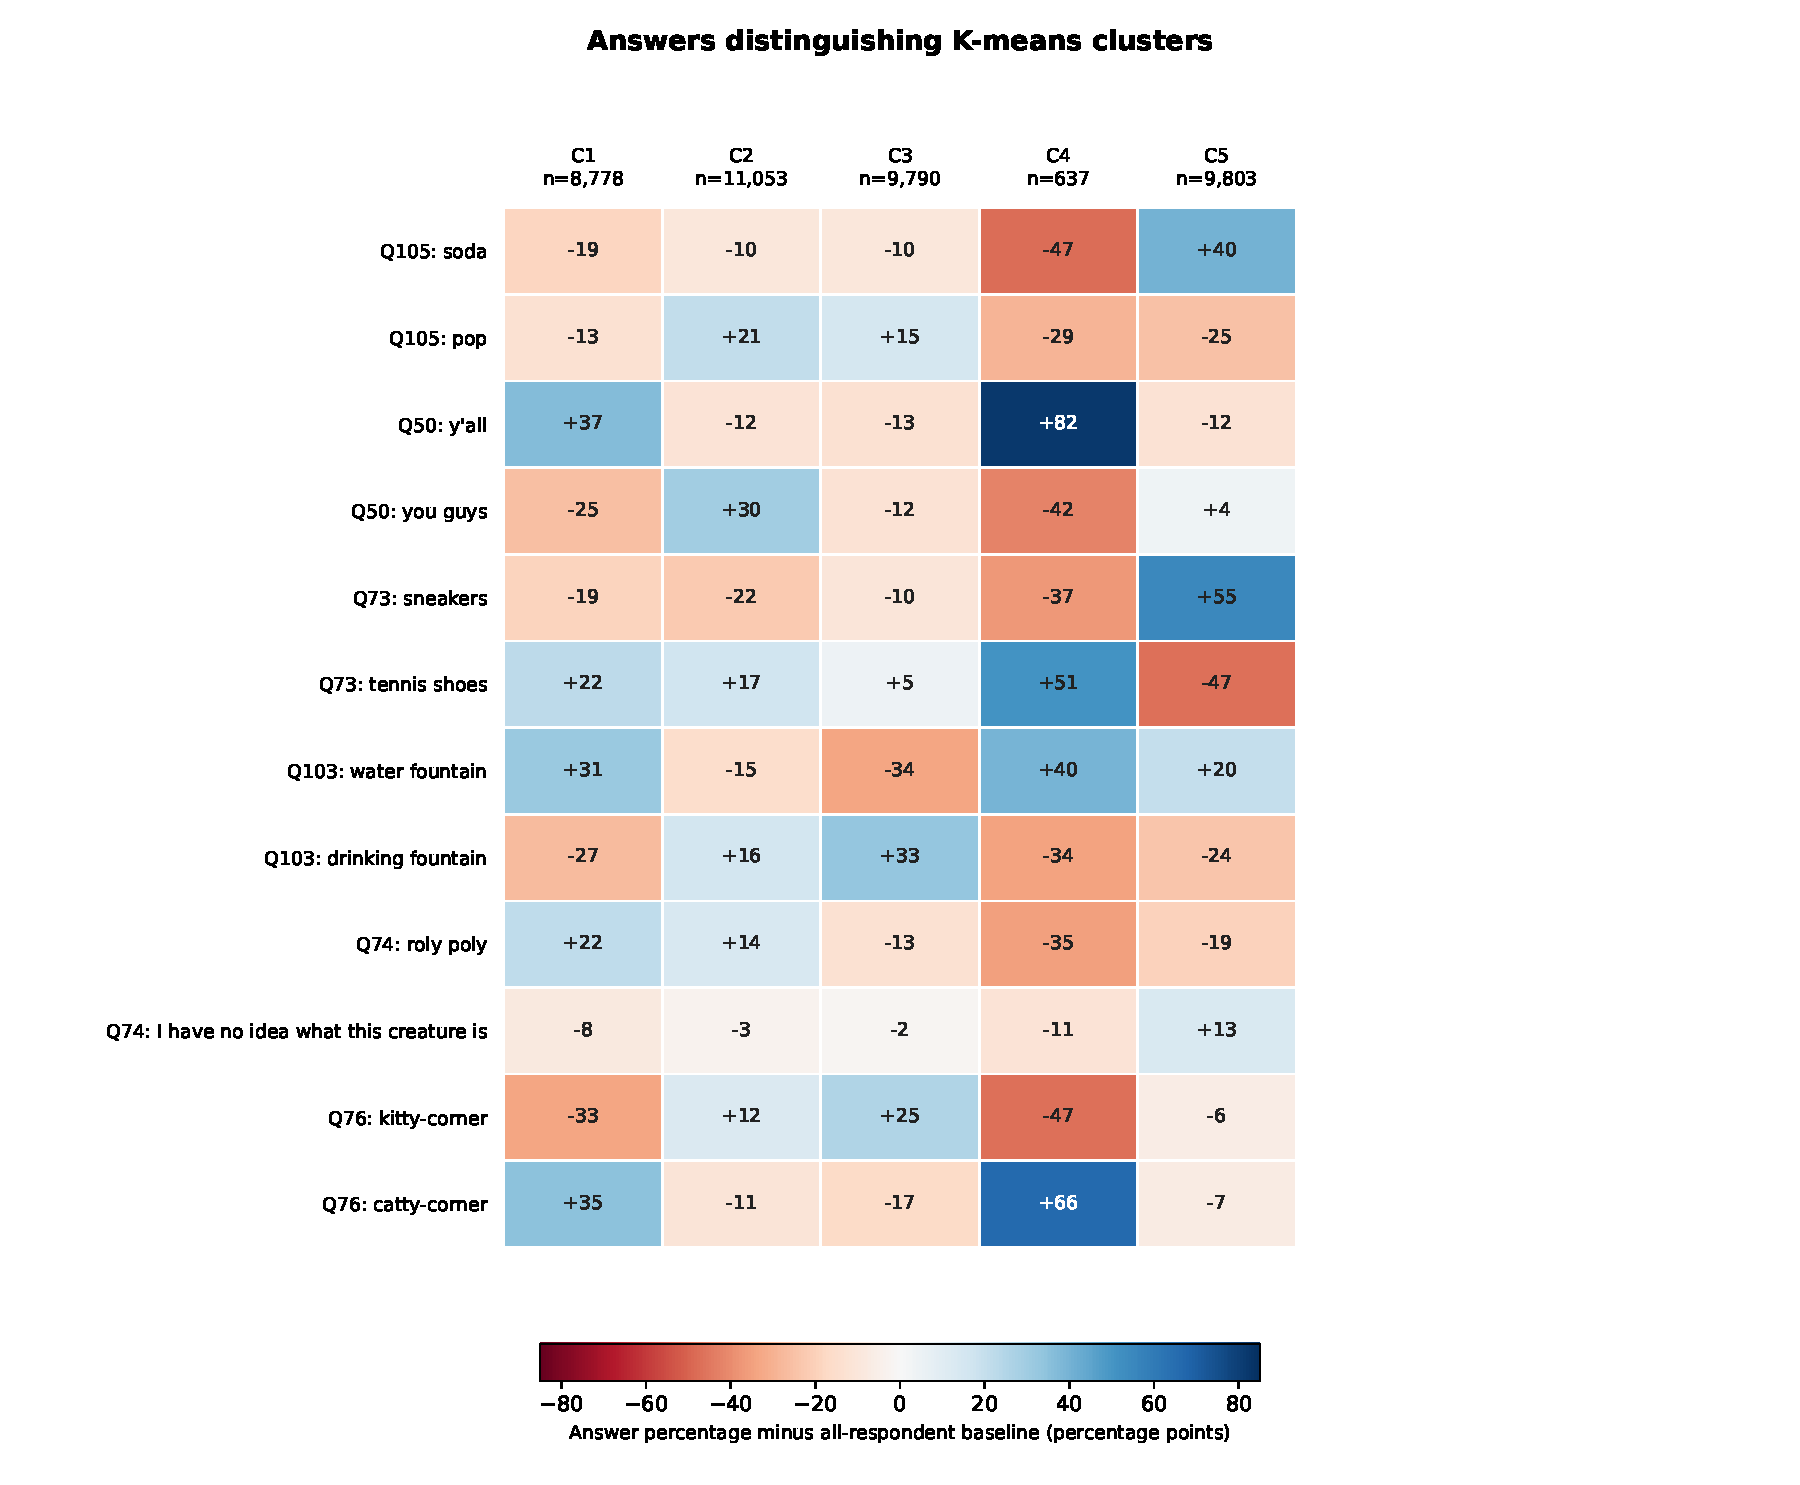
\includegraphics[width=\linewidth]{step4_kmeans_answer_profiles.pdf}
\caption{Selected K-means answer profiles. Values are percentage point differences from the overall baseline. A positive value means an answer is more common in that group.}
\label{fig:kmeans-profile}
\end{figure}

The clearest differences between the K-means groups are in Q105, which asks about soda, pop, and related terms. Other differences include how respondents address a group, what they call athletic shoes and drinking fountains, their answers to Q74, and their words for diagonally opposite street corners. In C5, soda is 40 percentage points above its baseline and sneakers is 55 points above the baseline. In C1, y'all, tennis shoes, and catty-corner are 37, 22, and 35 percentage points above their respective baselines.

C2 and C3 both use pop more often than the baseline, but their other answers help explain why K-means separates them. The percentage using \emph{you guys} is 30 percentage points above its baseline in C2, compared with 12 points below it in C3. The groups also differ in their use of drinking fountain and kitty-corner. This suggests that the split reflects several word choices rather than pop alone, although these differences do not establish whether the groups are stable or represent seperate regional dialects.

\subsection{GMM profiles and repeated answers}
GMM C5 again uses soda and sneakers more often, by 41 and 56 percentage points above the overall percentages. This pattern appears in both methods even though their overall divisions differ. GMM C1 is more common in the South and uses tennis shoes and water fountain more often. Its large C2 covers much of the Midwest and West.

\begin{figure}[ht]
\centering
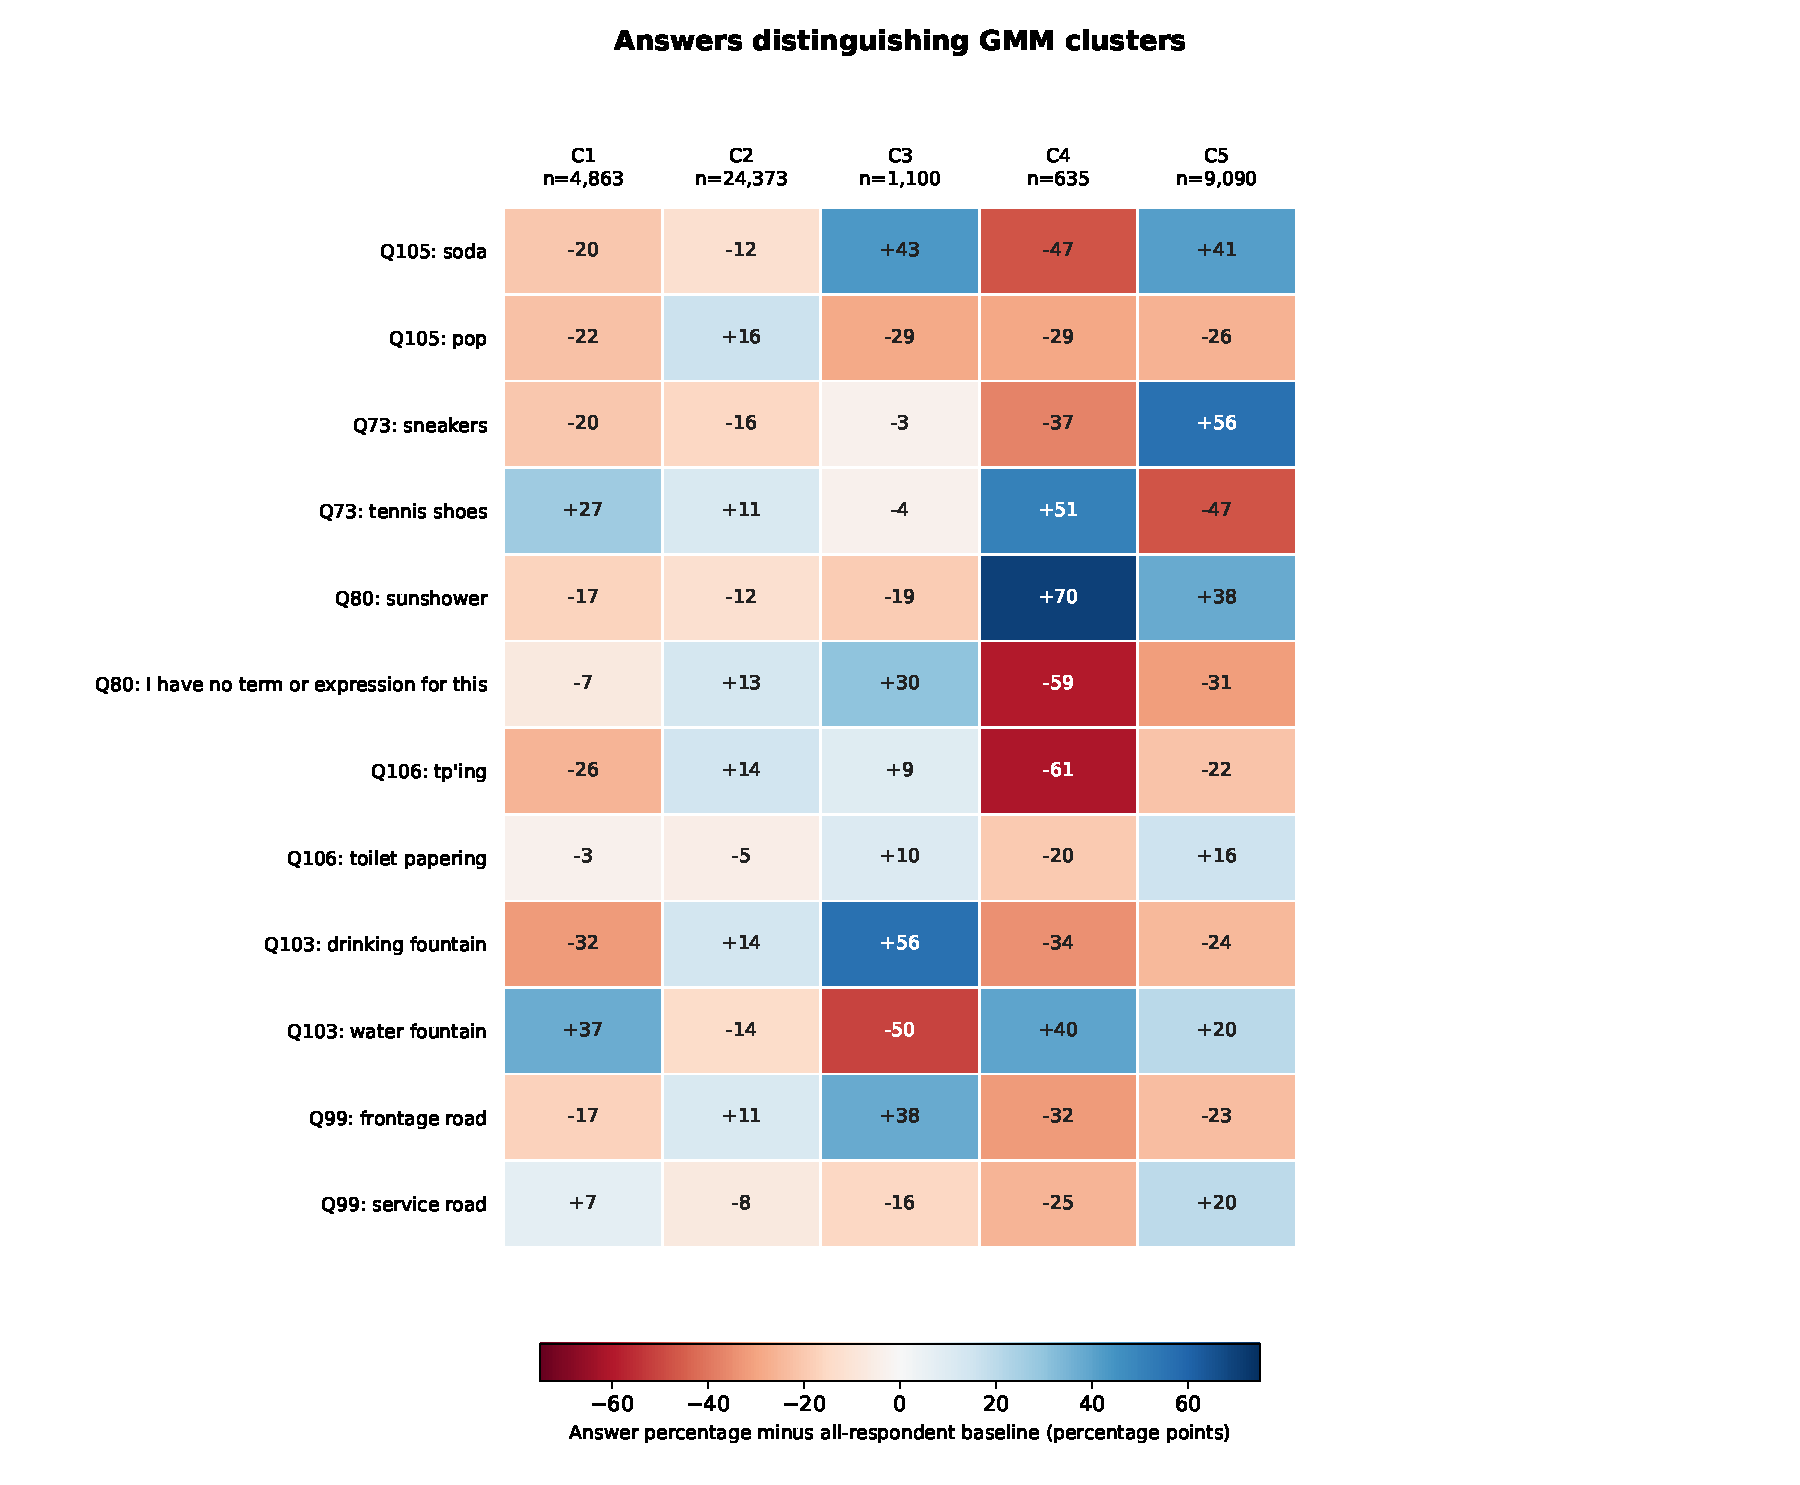
\includegraphics[width=\linewidth]{step4_gmm_answer_profiles.pdf}
\caption{Selected GMM answer profiles.}
\label{fig:gmm-profile}
\end{figure}

Together, the plots, maps, and answers suggest broad differences between the Northeast and interior, and between the South and northern/Western states. How the remaining respondents are grouped depends on the clustering method. These clusters show regional patterns, but their boundaries are not clear enough to define separate dialect regions.

\section{Stability of findings to perturbation}
The five-group K-means result is checked using 20 different seeds and 20 bootstrap samples. For the seed check, PCA is fixed and k-means is run with ten starts per fit. For each bootstrap, 40,061 people are drawn with replacement, then centered PCA is fit again with 50 components, and K-means is fit. This changes both the sample and the PCA representation.

Each fitted model is used to group all respondents and the groups are compared with Step 4 using the adjusted Rand index. This comparison is repeated for respondents left out of each bootstrap sample. This checks whether the results stay similar, not whether the dialect groups are correct. Individual groups are matched by their overlap using the Jaccard index. If a group splits or merges, the match may be poor.

\begin{center}
\begin{tabular}{lrrr}
\hline
Perturbation & ARI median & Minimum & Maximum\\
\hline
Different starts & 0.8847 & 0.7301 & 0.9222\\
Bootstrap, all respondents & 0.8847 & 0.4698 & 0.9523\\
Bootstrap, out-of-bag & 0.8883 & 0.4738 & 0.9548\\
\hline
\end{tabular}
\end{center}

\begin{figure}[ht]
\centering
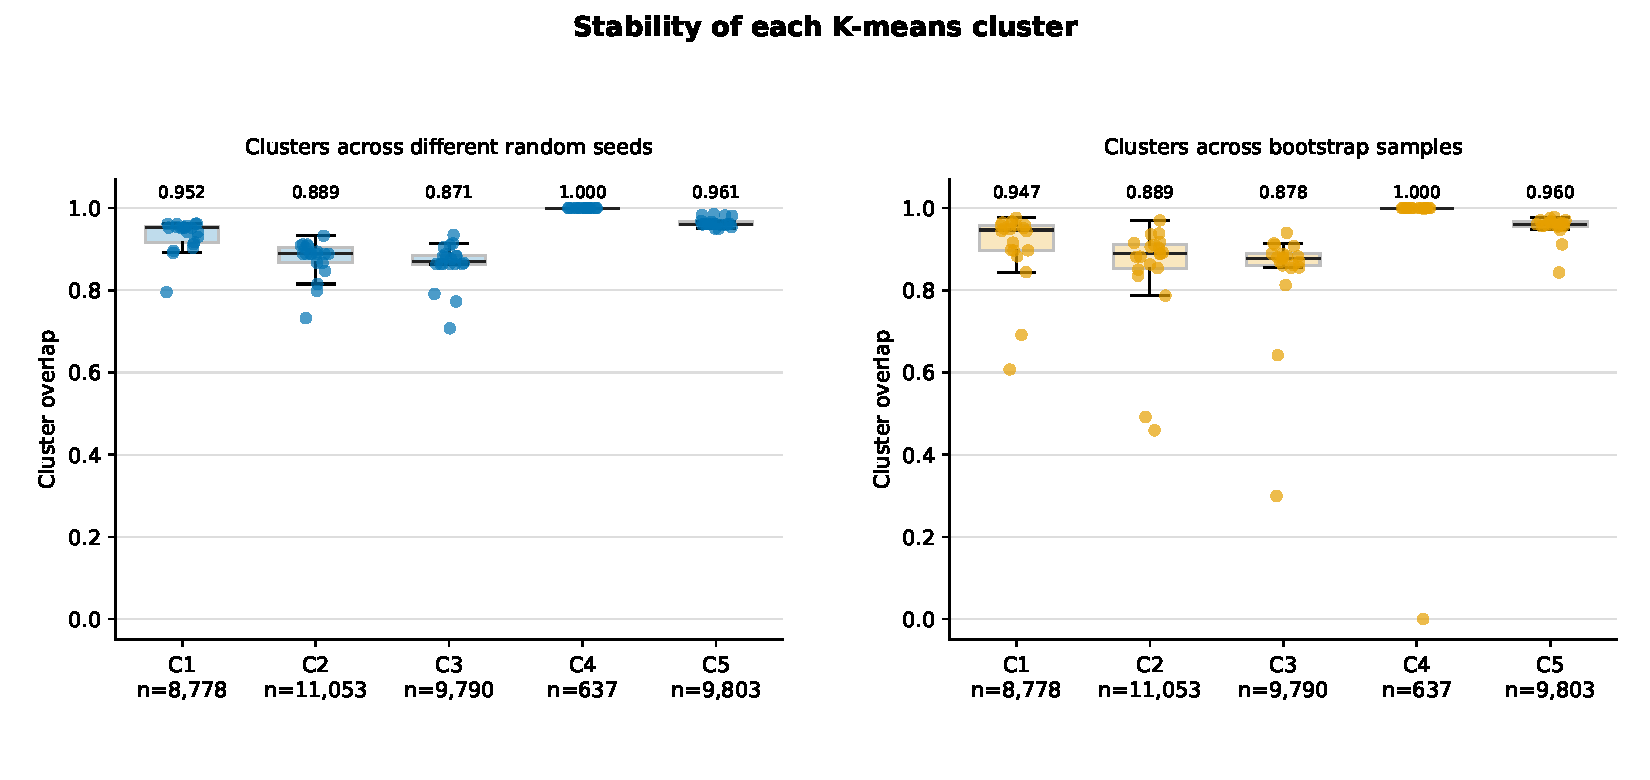
\includegraphics[width=\linewidth]{step5_kmeans_cluster_stability.pdf}
\caption{Jaccard overlaps across clusters for 20 runs. Numbers above groups are medians.}
\label{fig:stability}
\end{figure}

C5 is the most stable large group. Its bootstrap Jaccard median is 0.9603 and minimum 0.8434. The average change in its question-answer distributions has median 0.822\% and maximum 2.491\%. Its average regional-share change is 0.430 percentage points at the median and 2.128 at the maximum, across the four regions. This results support the Northeast soda/sneakers pattern more than an exact split of the middle.

C2 and C3 are less stable. Their lowest bootstrap overlaps are 0.4592 and 0.2996, and the weakest overall run has ARI 0.4698. C4 stays the same across different start fits, but its bootstrap median of 1.0 hides one zero-overlap match.

The broad answer patterns often repeat, but some runs differ greatly. The group count, PCA dimension, repeated-pattern weights, and treatment of missing answers have not been perturbed.

\section{Conclusion}
The findings depend on the data collected, the choices made during analysis, and how well the results apply to new data. This survey explores geographic word differences, but its results are not guaranteed to represent today's U.S. population. State averages also hide local differences and where people have lived before is not represented either.

The Northeast soda/sneakers group appears in both K-means and GMM and is relatively stable. Midwest/West divisions are less reliable. The group with repeated answers needs further investigation to understand why so many respondents gave the same answers. Checking different analysis choices and repeating the clustering can help show which findings are consistent.

These findings would possible be best used to guide language research or questionnaire design, rather than determining verified dialects. A reality check could use an independent survey with similar questions. I would apply the existing PCA and group centers, then check whether the same answer patterns and geographic differences appear.

With more time, I would compare people who did and did not answer everything, vary the numbers of PCs and groups, and more closely inspect repeated patterns. I would also look at smaller geographic areas, since state boundaries could hide certain patterns, and word use likely does not follow state boundaries.

\section{Academic Honesty}\label{honesty}

Dear Bin,

Academic honesty matters to me because dishonest or misrepresented work makes academic communication and scientific progress less efficient. I want to contribute to making the world better, so I feel that it is my responsibility to be academically honest.

I used Codex to review code and results, add docstrings and comments, refine the report at paragraph level, and to ensure that lab tasks were being sufficiently completed.

\subsection{Collaborators}
I did not work with any human collaborators.

\begin{thebibliography}{3}
\bibitem{nerbonne2003}
J. Nerbonne and W. Kretzschmar.
Introducing Computational Techniques in Dialectometry.
\emph{Computers and the Humanities}, 37(3), 245--255, 2003.
\href{https://doi.org/10.1023/A:1025064105053}{doi:10.1023/A:1025064105053}.

\bibitem{nerbonne2006}
J. Nerbonne and W. Kretzschmar Jr.
Progress in Dialectometry: Toward Explanation.
\emph{Literary and Linguistic Computing}, 21(4), 387--397, 2006.
\href{https://doi.org/10.1093/llc/fql034}{doi:10.1093/llc/fql034}.

\bibitem{survey}
B. Vaux. Dialect Survey, course-provided response data and question metadata.
STAT 215A Lab 2 materials, Fall 2026.
\url{https://www.dialectsofenglish.com/}. Survey attribution and file processing history follow the course instructions.

\end{thebibliography}
\end{document}